% Options for packages loaded elsewhere
\PassOptionsToPackage{unicode}{hyperref}
\PassOptionsToPackage{hyphens}{url}
\PassOptionsToPackage{dvipsnames,svgnames,x11names}{xcolor}
%
\documentclass[
  11pt,
]{book}
\usepackage{amsmath,amssymb}
\usepackage{lmodern}
\usepackage{iftex}
\ifPDFTeX
  \usepackage[T1]{fontenc}
  \usepackage[utf8]{inputenc}
  \usepackage{textcomp} % provide euro and other symbols
\else % if luatex or xetex
  \usepackage{unicode-math}
  \defaultfontfeatures{Scale=MatchLowercase}
  \defaultfontfeatures[\rmfamily]{Ligatures=TeX,Scale=1}
\fi
% Use upquote if available, for straight quotes in verbatim environments
\IfFileExists{upquote.sty}{\usepackage{upquote}}{}
\IfFileExists{microtype.sty}{% use microtype if available
  \usepackage[]{microtype}
  \UseMicrotypeSet[protrusion]{basicmath} % disable protrusion for tt fonts
}{}
\makeatletter
\@ifundefined{KOMAClassName}{% if non-KOMA class
  \IfFileExists{parskip.sty}{%
    \usepackage{parskip}
  }{% else
    \setlength{\parindent}{0pt}
    \setlength{\parskip}{6pt plus 2pt minus 1pt}}
}{% if KOMA class
  \KOMAoptions{parskip=half}}
\makeatother
\usepackage{xcolor}
\usepackage[margin=1in]{geometry}
\usepackage{longtable,booktabs,array}
\usepackage{calc} % for calculating minipage widths
% Correct order of tables after \paragraph or \subparagraph
\usepackage{etoolbox}
\makeatletter
\patchcmd\longtable{\par}{\if@noskipsec\mbox{}\fi\par}{}{}
\makeatother
% Allow footnotes in longtable head/foot
\IfFileExists{footnotehyper.sty}{\usepackage{footnotehyper}}{\usepackage{footnote}}
\makesavenoteenv{longtable}
\usepackage{graphicx}
\makeatletter
\def\maxwidth{\ifdim\Gin@nat@width>\linewidth\linewidth\else\Gin@nat@width\fi}
\def\maxheight{\ifdim\Gin@nat@height>\textheight\textheight\else\Gin@nat@height\fi}
\makeatother
% Scale images if necessary, so that they will not overflow the page
% margins by default, and it is still possible to overwrite the defaults
% using explicit options in \includegraphics[width, height, ...]{}
\setkeys{Gin}{width=\maxwidth,height=\maxheight,keepaspectratio}
% Set default figure placement to htbp
\makeatletter
\def\fps@figure{htbp}
\makeatother
\setlength{\emergencystretch}{3em} % prevent overfull lines
\providecommand{\tightlist}{%
  \setlength{\itemsep}{0pt}\setlength{\parskip}{0pt}}
\setcounter{secnumdepth}{5}
\usepackage{booktabs}
\ifLuaTeX
  \usepackage{selnolig}  % disable illegal ligatures
\fi
\usepackage[]{natbib}
\bibliographystyle{plainnat}
\IfFileExists{bookmark.sty}{\usepackage{bookmark}}{\usepackage{hyperref}}
\IfFileExists{xurl.sty}{\usepackage{xurl}}{} % add URL line breaks if available
\urlstyle{same} % disable monospaced font for URLs
\hypersetup{
  pdftitle={Transforming Research Methods in Health Services Psychology: Applications for the Advocate \textasciitilde{} Practitioner \textasciitilde{} Scientist},
  pdfauthor={Lynette H. Bikos, PhD, ABPP \& Cirleen DeBlaere, PhD, Editors; Kiana Clay, Editorial Assistant},
  colorlinks=true,
  linkcolor={Maroon},
  filecolor={Maroon},
  citecolor={Blue},
  urlcolor={blue},
  pdfcreator={LaTeX via pandoc}}

\title{Transforming Research Methods in Health Services Psychology: Applications for the Advocate \textasciitilde{} Practitioner \textasciitilde{} Scientist}
\author{Lynette H. Bikos, PhD, ABPP \& Cirleen DeBlaere, PhD, Editors \and Kiana Clay, Editorial Assistant}
\date{02 Aug 2022}

\begin{document}
\maketitle

{
\hypersetup{linkcolor=}
\setcounter{tocdepth}{3}
\tableofcontents
}
\hypertarget{book-cover}{%
\chapter*{BOOK COVER}\label{book-cover}}
\addcontentsline{toc}{chapter}{BOOK COVER}

\begin{figure}
\centering
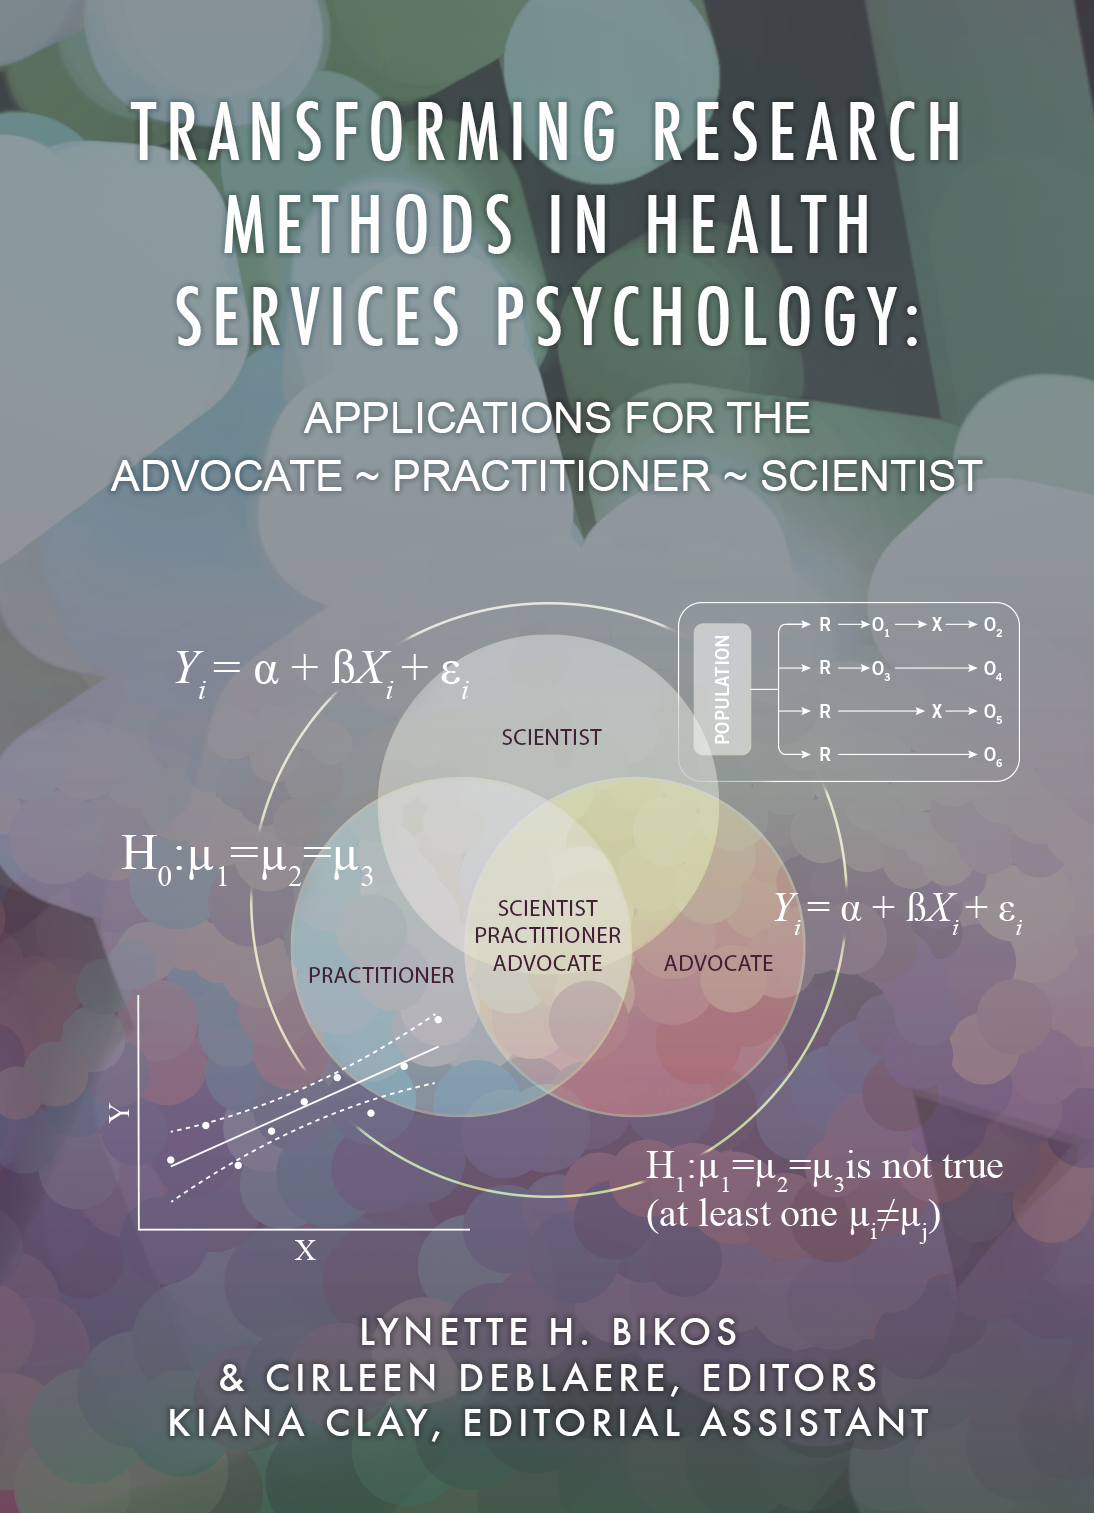
\includegraphics{images/bookcover.png}
\caption{An image of the book cover. It includes three overlapping, pastel-colored, circles representing advocacy, practice, and science. These are surrounded by a handful of statistical symbols and formulae. methods.}
\end{figure}

This open education resource is available in the following formats, all available in the \href{https://github.com/lhbikos/TransformingResearchMethods/tree/main/docs}{docs} folder at the GitHub repository:

\begin{itemize}
\tightlist
\item
  Formatted as an \href{https://lhbikos.github.io/TransformingResearchMethods/}{html book} via GitHub Pages available
\item
  As a \href{https://github.com/lhbikos/TransformingResearchMethods/blob/main/docs/TransformingResearchMethods.pdf}{PDF}
\item
  As an \href{https://github.com/lhbikos/TransformingResearchMethods/blob/main/docs/TransformingResearchMethods.epub}{ebook}
\item
  As a \href{https://github.com/lhbikos/TransformingResearchMethods/blob/main/docs/TransformingResearchMethods.docx}{Word Document}
\end{itemize}

All materials used in creating this OER are available at its \href{https://github.com/lhbikos/TransformingResearchMethods}{GitHub repo}.

\hypertarget{preface}{%
\chapter*{PREFACE}\label{preface}}
\addcontentsline{toc}{chapter}{PREFACE}

\textbf{If you are viewing this document, you should know that this is a book-in-progress. Early drafts are released for the Transforming Counseling Psychology Curriculum Showcase at APA 2022, for peer review, and for generating interest in collaboration. The document was last updated on 02 Aug 2022}.

In her 2021-2022 term as President of the Society of Counseling Psychology, one of Dr.~Amy Reynolds' Presidential Initiatives was \emph{Transforming Counseling Psychology Curriculum and Praxis.} Dr.~Reynolds invited counseling psychology faculty, practitioners, and doctoral students ``to critically examine and deconstruct how various competencies, courses, and content are taught; how we socialize our students; and then re-imagine, dream, and reconstruct new and transformative ways to teach and train.''

\hypertarget{strategies-for-a-social-responsivity}{%
\section*{Strategies for a Social Responsivity}\label{strategies-for-a-social-responsivity}}
\addcontentsline{toc}{section}{Strategies for a Social Responsivity}

This open education resource (OER) is a product of the group devoted to \emph{research}. There are a number of strategies we used to ensure that the OER moves in the direction of being socially and culturally responsive.

\begin{itemize}
\tightlist
\item
  Our authors committed to using the guidelines for a liberated syllabus found in the CCTC: Social Responsiveness in \href{https://pr4tb8rrj317wdwt3xlafg2p-wpengine.netdna-ssl.com/wp-content/uploads/2021/05/CCTC_Socially-Responsive-HSP-Ed-Training_v7.pdf}{Health Services Psychology Education \& Training Toolkit}.
\item
  We chose the format of OER because provides a zero-cost \emph{textbook} to faculty and students.
\item
  We sought authors and co-author teams that represent the diversity of health services psychology including discipline (counseling, clinical, educational),stage in career (students, early career professionals, mid- and late- career professionals), and identities that have been marginalized in higher education and our discipline.
\item
  Each chapter works its way through an open peer review process where the chapter (with authors clearly identified)is hosted in a shared drive. At least two reviewers can mark up the same document and contribute to the same rubric. At any time the author(s) can see the review and, if desired, dialogue with the reviewers. At the outset, we specified the tone to be ``formative not summative.''
\item
  Although we are still learning, we have attempted to use tools and techniques that are consistent with universal design. For example, we hope that the image captions and headers are marked such that text readers will identify them as such.
\end{itemize}

\hypertarget{perpetually-in-progress}{%
\section*{Perpetually in Progress}\label{perpetually-in-progress}}
\addcontentsline{toc}{section}{Perpetually in Progress}

This book is being formatted in R Markdown, rendered into its ``book'' format with Bookdown, hosted on GitHub, and pushed to the internet (in its html format) through GitHub Pages. This set of tools allows the book to be \emph{perpetually-in-progress.} This means that our authors can update their chapters at-any-time. It also means that we can add chapters at-any-time. If you are interested in contributing to the book, please contact us. It is one of our greatest hopes that this flexibility contributes to the socially and culturally responsive pedagogy that we intend.

\hypertarget{under-construction}{%
\section*{Under Construction}\label{under-construction}}
\addcontentsline{toc}{section}{Under Construction}

At this stage in the OER's development, authors are still writing and revising chapters. The following designations will identify the chapters that have not been through the review process:

\begin{itemize}
\tightlist
\item
  \emph{In-progress} means that the chapter is partially written (or perhaps outlined) and that the author(s) are continuing to work on the chapter.
\item
  \emph{Under review} means that the chapter is being (or has been) peer-reviewed.
\end{itemize}

\hypertarget{acknowledgements}{%
\section*{Acknowledgements}\label{acknowledgements}}
\addcontentsline{toc}{section}{Acknowledgements}

Financial support, supporting the copy editing and desktop publishing for this project was provided by the Office of Education, Technology, \& Media, Seattle Pacific University (Summer 2022).

The book cover was designed by Dominic Williamson, Senior Instructional Designer in Graphics \& Illustrations, in the Office of Education, Technology, \& Media at Seattle Pacific University.

\hypertarget{copyright-with-open-access}{%
\section*{Copyright with Open Access}\label{copyright-with-open-access}}
\addcontentsline{toc}{section}{Copyright with Open Access}

This book is published under a a Creative Commons Attribution-NonCommercial-ShareAlike 4.0 International License. This means that this book can be reused, remixed, retained, revised and redistributed (including commercially) as long as appropriate credit is given to the authors. If you remix, or modify the original version of this open textbook, you must redistribute all versions of this open textbook under the same license - CC BY-SA.

A \href{https://github.com/lhbikos/ReC_MultivModel}{GitHub open-source repository} contains all of the text and source code for the book, including data and images.

\hypertarget{InExVal}{%
\chapter{Internal and External Validity in Health Service Psychology}\label{InExVal}}

\emph{Franco Dispenza, PhD (he/him/his) \& Alec Prince, MPA}\\
\emph{Georgia State University}\\
\emph{Georgia State University is located on the traditional homelands of the Muscogee Creek and Cherokee Nations}

The focus of this lesson is to provide a review of internal validity, external validity, threats to validity, and current trends and considerations in relation to validity. Internal and external validity are foundational to experimental and quasi-experimental research. In experimental and quasi-experimental research designs, health service psychologists work thoughtfully and diligently to ensure that a line of systematic inquiry demonstrates some degree of internal and external validity. This is because psychologists and behavioral health researchers are concerned with making reasonable epistemological claims that could directly impact the lives of diverse communities and populations, especially in research studies attempting to show if particular interventions, treatments, or programs have a true effect on specific outcomes.

Whereas researchers utilizing qualitative frameworks may be more interested in methodological integrity (e.g., credibility and transferability; Levitt et al., 2017), researchers employing quantitative-based paradigms are especially interested in internal and external validity. You will notice that the term ``validity'' is used in many concepts and research frameworks, including construct validity, content validity, predictive validity, criterion validity, and statistical conclusion validity. These are all specific types of validity attempting to establish a degree of accuracy or truthfulness in research. Further, the aforementioned forms of validity often have statistical computations and procedures that accompany them (e.g., bivariate correlations, beta weights, etc.). This chapter will not address those forms of validity. Instead, we will focus on internal and external validity, conceptual constructs that rely on methodological procedures and considerations versus statistical calculations.

\hypertarget{learning-objectives}{%
\section{Learning Objectives}\label{learning-objectives}}

Learning objectives for this chapter include the following:

\begin{itemize}
\tightlist
\item
  Students will be able to explain the dimensional features of internal and external validity in experimental and quasi-experimental research.
\item
  Students will be able to list and discuss threats associated with internal and external validity in experimental and quasi-experimental research.
\item
  Students will be able to discuss and apply established methods for controlling the various threats associated with internal and external validity in experimental and quasi-experimental research.
\item
  Students will be able to identify and apply their knowledge of internal validity, external validity, and their associated threats to current trends and issues in psychological research.
\item
  Students will be able to critique and distinguish the strengths and limitations of internal and external validity when applied to socially responsive research.
\end{itemize}

\hypertarget{recommended-readings}{%
\section{Recommended Readings}\label{recommended-readings}}

The following served as critical references in the development of this chapter. We encourage you to review them.

\begin{itemize}
\tightlist
\item
  Campbell, D. T., \& Stanley, J. C. (1963). Experimental and quasi- experimental designs for research. Chicago, IL: Rand McNally.
\end{itemize}

This classic and foundational text introduces readers to internal validity, external validity, and threats to validity as originally proposed by Campbell and Stanley. It also provides readers with an overview of the various experimental and quasi-experimental methodological designs, and how various methodological designs could be used to minimize threats to validity.

\begin{itemize}
\tightlist
\item
  Ferguson L. (2004). External validity, generalizability, and knowledge utilization. \emph{Journal of Nursing Scholarship, 36}(1), 16-22. \url{https://doi.org/10.1111/j.1547-5069.2004.04006.x}
\end{itemize}

Although aimed for a nursing audience, there is much to be gained from Ferguson's (2004) review of external validity, generalizability, and evidence-based practice. Ferguson reviews much of the major conceptual tenets of external validity, including its threats and control strategies. Ferguson also discusses ways in which researchers and practitioners could enhance external validity of research.

\begin{itemize}
\tightlist
\item
  Schmuckler, M.A.~(2001).What Is Ecological Validity? A Dimensional Analysis. \emph{Infancy, 2}(4), 419-436. \url{https://doi.org/10.1207/S15327078IN0204_02}
\end{itemize}

Schmuckler (2001) introduces readers to a subset of external validity, namely ecological validity. Schmuckler provides an historical review of ecological validity, and a discussion of the various dimensions, advantages, and criticisms of ecological validity.

\hypertarget{internal-validity}{%
\section{Internal Validity}\label{internal-validity}}

Health service psychologists are committed to accuracy, honesty, and truthfulness when engaging in the research process. Whether representing research findings fairly, capturing the essence of people's lived experiences with precision, or using research to advocate against harmful psychological practices, researchers are compelled to uphold the integrity of the knowledge claims they make through their scholarship. Researchers are committed to ensuring that their research is justifiable, well-grounded, and internally valid.

\emph{Internal validity} is the extent to which a researcher can infer cause-effect relationships between a set of variables, while simultaneously excluding the influence of confounding or extraneous variables (Campbell \& Stanley, 1963; Cook \& Campbell, 1979). In an attempt to establish internal validity, it is important to rule out the effects of confounding or extraneous variables. \emph{Confounding or extraneous variables} can serve as potential rivals to inferred relationships, leading a researcher to be less confident about the conclusions and implications that can be made between an independent (or treatment) variable and a dependent (or outcome) variable.

\emph{Methodological control} is also paramount in experimental and quasi-experimental research. In an ideal research scenario, a researcher will have identified and controlled for all possible confounds and extraneous variables that may be inherent in the methodological design of a study. Since determining causality is the goal in experimental and quasi-experimental research, such a scenario would render a study to be high in internal validity. However, we know in practice there is no such thing as a perfect study, especially when there exist numerous \emph{threats to internal validity}. Threats consist of factors or conditions that endanger a researcher's capacity to amplify a study's level of internal validity (Onwuegbuzie \& McLean, 2003).

\hypertarget{threats-to-internal-validity}{%
\subsection{Threats to Internal Validity}\label{threats-to-internal-validity}}

Researchers often execute considerable forethought when identifying and eliminating potential threats to internal validity. Psychological researchers are encouraged to use a variety of logic-informed heuristics, ``what if'' sensitivity analyses, or consider any new data or findings to rule out rival hypotheses (Kenny, 2019). Researchers are also encouraged to consider more classically identified threats to their research design (Campbell \& Stanley, 1963). Some of the most common threats to internal validity consist of history, maturation, instrumentation, statistical regression, selection, attrition, and experimenter bias (Campbell \& Stanley, 1963; Cook \& Campbell, 1979; Shadish et al., 2002). Threats to internal validity can occur, or be discovered, at any point during the research process, including design, implementation, data collection, and analyses. There can exist multiple threats in a given study, and these threats can also intersect with one another. Keep in mind that threats are never something a researcher just ``checks off'' in a box, but rather a researcher continuously monitors their methods to ensure the credibility of the concluded findings (Onwuegbuzie \& McLean, 2003). Each threat to internal validity is discussed in more detail below.

\hypertarget{history}{%
\subsubsection{History}\label{history}}

No researcher can control the potential of geological, sociopolitical, financial, cultural, climate-related, pandemic, and other national and global events from impacting individuals in a research study. But inevitably such events happen, and unfortunately with what seems to be at higher frequencies these days. Historical events can influence the manner in which participants respond to a study's dependent variable, making it difficult for researchers to determine whether an observed outcome was the result of a study's independent variable or the historical event. In some instances, the historical event could directly intersect with objectives of the study itself making it even more difficult for researchers to make valid conclusions. Imagine you are evaluating the effectiveness of a new stress-reduction intervention for survivors of catastrophic hurricanes in a low-income, rural community in the southeast United States. In the middle of implementing the intervention, a tornado hits the same community, leading to severe damage and loss of life. What impact will this historical event have on the research study?

\hypertarget{maturation}{%
\subsubsection{Maturation}\label{maturation}}

Development and growth are natural processes that occur for individuals during their lifespan. These processes could be physiological, cognitive, social, or emotional. Given the length of a particular study, sometimes results from a study may be more indicative of naturally occurring growth and developmental factors, versus any manipulated independent variable.

\hypertarget{instrumentation}{%
\subsubsection{Instrumentation}\label{instrumentation}}

No tool, test, or measure used in research can be entirely valid and reliable one hundred percent of the time. Instruments can produce low reliability scores or even produce inadequate psychometric properties (e.g., construct and predictive validity) with a study's particular sample. This is an important consideration as some tests and measures were never validated or normed with diverse samples. Consider a measure of marital satisfaction that was created using heterosexual couples in the Netherlands. The measure may have great face validity, and even demonstrate adequate levels of content, criterion, and construct validity. But it may not produce the same psychometrics if used in married couples in the United States. It may be entirely inappropriate to use this measure if the United States sample also includes same-sex couples. Lastly, human beings administering instruments could contribute additional error, making instrumentation a serious threat to research studies. For example, some researchers may become fatigued when administering some measures, may not be consistent with measurement, or may not accurately observe a phenomenon during a research study.

\hypertarget{testing}{%
\subsubsection{Testing}\label{testing}}

It is common to test participants multiple times throughout the course of a research study. Researchers often use the same test, measure, scale, or inventory when testing participants, but it begs the question as to whether changes in a test---that had been given multiple times---reflect true change? Sometimes referred to either as a \emph{practice effect} or \emph{fatigue effect}, changes in scores on the same test may be the result of familiarity with the test or becoming tired with the test.

\hypertarget{statistical-regression-or-regression-to-the-mean}{%
\subsubsection{Statistical Regression, or Regression to the Mean}\label{statistical-regression-or-regression-to-the-mean}}

Sometimes researchers select participants based on high or low scores on a particular test or measure (Campbell \& Kenny, 1999). For example, researchers may be interested in examining people who score high on measures of academic or cognitive functioning. If retested, those same participants may continue to score high or low. However, not all would score as high or low because of statistical regression, or regression to the mean. When participants are retested, researchers find that scores are less extreme and center toward an average score. Imagine a researcher was interested in testing a career counseling intervention with first generation college students who reported high scores on career indecision and anxiety in a career battery of questionnaires. After the intervention is complete, the researchers issue a final battery of questionnaires. These same first generation college students may appear less anxious and indecisive due to statistical regression to the mean and not necessarily the intervention.

\hypertarget{attrition-or-differential-mortality}{%
\subsubsection{Attrition, or Differential Mortality}\label{attrition-or-differential-mortality}}

Ethically, participants have the right to withdraw from participating in a research study at any given time during the research process. When participants withdraw, or drop from a study, researchers refer to this as attrition. A major concern of attrition is that it leads to potential biases in scores between groups (or observations in the case of longitudinal studies) that may not reflect whether an independent variable had any effect on the dependent variable. If there is substantial attrition in one group, or across the entire study, it leads a researcher to question why participants are withdrawing. Researchers may further wonder if participants dropping from the study are characteristically different from those who are remaining in the study. Attrition limits the type of conclusions that can be made because observations made across time or between groups may not reflect true differences as a function of the independent variable. Rather, there may be some other underlying issue with the research study.

Imagine a researcher has been evaluating the effects of a six-session mindfulness cognitive behavioral group intervention for the reduction of race related stress among Black and African American women employed in a large healthcare setting. The researcher used a longitudinal, between group experimental design with an intervention group (treatment) and a control group (education), but found that attrition rates were higher for those in the control than for the intervention group. Equivalent and adequate comparisons could not be reliably made between the two groups at completion of study, so the researcher decided to send surveys to those dropped from the study and inquire why they dropped. The surveys return and the researcher finds that a significant portion of the control group were made up of on-call, ambulatory nurses who were unable to commit to the scheduled sessions. Therefore, the attrition was the result of some characteristic that differentiated the two groups.

\hypertarget{experimenter-bias}{%
\subsubsection{Experimenter Bias}\label{experimenter-bias}}

Researchers need to ensure they do not engage in verbal or nonverbal behaviors that inadvertently alter the results of a study. Sometimes this is referred to as an \emph{experimenter expectancy}, and it is even known as the \emph{Rosenthal Effect}. This becomes a threat when a participant's response in a study is the result of the experimenter's expectations versus the manipulated or independent variable. Examples include emphasizing particular words when reading prompts or scripts, or excessive nodding and smiling when certain favorable responses are solicited by study participants.

\hypertarget{selection-bias}{%
\subsubsection{Selection Bias}\label{selection-bias}}

Differences between groups in experimental studies can sometimes be the result of characteristics of the participants themselves, versus the manipulated or independent variable. For instance, a researcher may have accidentally grouped people along the same characteristic, such as sex, gender, sexual orientation, race, ethnicity, or age group. This potentially sets up nonequivalent groups in experimental or quasi-experimental research, and makes it difficult for researchers to determine whether any changes in dependent or outcome variables were the result of an independent variable or the characteristic itself. This also pertains to self-selection bias commonly seen in survey and questionnaire research, in which participants self-select to participate in a study.

\hypertarget{controlling-for-threats-to-internal-validity}{%
\subsection{Controlling for Threats to Internal Validity}\label{controlling-for-threats-to-internal-validity}}

Researchers have identified a number of methodological procedures that could be used to control for threats to internal validity (Campbell \& Stanley, 1963; Cook \& Campbell, 1979; Fabrigar et al., 2020; Onwuegbuzie \& McLean, 2003; Shadish et al., 2002). Below we discuss the importance of considering control groups, random assignment, matching, blocking and holding variables constant.

\hypertarget{control-groups}{%
\subsubsection{Control Groups}\label{control-groups}}

Control groups are commonly used in experimental and quasi-experimental human subjects research, and there is an important logic to its use. Individuals are assigned to a group (or condition) in which they do not receive the treatment or manipulated variable. However, participants do partake in similar tasks and conditions (e.g., complete surveys, questionnaires, physiological markers, etc.) as those in the experimental condition. Upon completion of the study, researchers then compare how the intervention or experimental condition performed alongside the control condition or group. Control groups are particularly effective at controlling for the effects of history, maturation, testing, instrumentation, and regression toward the mean (Campbell \& Stanley, 1963; Cook \& Campbell, 1979).

\hypertarget{random-assignment}{%
\subsubsection{Random Assignment}\label{random-assignment}}

Considered one of the most robust methods to control against threats to internal validity, researchers randomly place volunteer participants in various study conditions at the very beginning of a research study. This assures the researcher that each participant had the same or equally probable chance of being placed in either an experimental condition (or group) or a control condition (or group), while helping to decrease any unknown or intentional influence on assignment of participants to different groups. It further assures the researcher that the groups are equitable in terms of various characteristics of the participants (e.g., demographics, temperament, etc.; Fabrigar et al., 2020). Any observed differences or changes seen among the groups or conditions could then be accounted for by the manipulated independent variable or the applied intervention. More importantly, any observed difference between the groups is not the result of any sort of systematic bias that might have occurred during the initial phases of the research study.

Take a hypothetical scenario in which a researcher is evaluating the ways in which implicit sexist messaging influences women's responses to a cognitive motor task. Women are recruited from the community to participate in the study. One group receives the implicit sexist messaging while the other group does not. However, nearly all members in one group happened to be women between the ages of 21 and 29, while the majority of those in another group were women between the age of 43 and 56 This could constitute a systematic bias since there are generational differences between members in one group versus the other. Random assignment is incredibly important when controlling for the effects of selection (Campbell \& Stanley, 1963; Cook \& Campbell, 1979; Shadish et al., 2002).

It is important to keep in mind that random assignment and random sampling are not synonymous with one another. \textbf{Random sampling} is when researchers utilize a variety of probable sampling techniques (e.g., simple, systematic, stratified, or cluster) to recruit participants who approximate the general population. It also means that all members of a given population have an equal chance of being recruited to participate.

\hypertarget{matching}{%
\subsubsection{Matching}\label{matching}}

To further avoid the threat of selection bias, researchers may engage in the process of participant matching. This is especially helpful if a researcher cannot guarantee equivalent groups through randomization, or when sample size may be too small. Participants are matched on a variety of characteristics (e.g., cognitive or intelligence pre-test scores, gender, age, etc.), by placing members of similar characteristics in either an experimental/intervention condition or in the control condition. This helps a researcher establish some degree of equivalence between groups within a particular sample.

\hypertarget{blocking-and-holding-variables-constant}{%
\subsubsection{Blocking and Holding Variables Constant}\label{blocking-and-holding-variables-constant}}

Researchers may also choose to use some characteristic in the study's sample (e.g., cognitive or intelligence scores, ethnicity or race) as an additional independent variable. This is referred to as \emph{blocking}. Unlike matching, researchers may employ this strategy to see if a particular characteristic of the sample has an effect on the dependent variable. Alternatively, some researchers may choose to hold a particular characteristic constant or homogenize some sample characteristic so as to eliminate any undue influence from extraneous characteristics of a sample. For instance, a researcher may choose to only recruit high school aged adolescent boys between the ages of 14 and 15 who score above a certain threshold on an anxiety and depression measure to participate in a short-term emotional regulation treatment study.

\hypertarget{external-validity}{%
\section{External Validity}\label{external-validity}}

Many researchers invest time and resources with the hopes of expanding their research findings to larger communities and contexts, especially if the research is aimed at alleviating any suffering or influence larger systemic change efforts. Thus, researchers are not only concerned with internal validity, but also the external validity of their study. \textbf{External validity} is the degree towhich research findings can be generalized to the population that approximate the original context of the study (Campbell \& Stanley, 1963; Cook \& Campbell, 1979; Shadish et al., 2002).

External validity is also concerned with the degree in which a study can be generalized across broader populations, treatments, settings, and conditions (Ferguson, 2004). Researchers wish to move beyond the controlled setting in which the study originally took place, and further consider ways that the findings may apply in other diverse applicational settings, time, persons, or slightly different variables or targets (Kenny, 2019; Shadish et al., 2002). For instance, a researcher who evaluated the effectiveness of a minority stress reduction intervention for transgender and gender nonbinary individuals in a controlled laboratory setting at a university, might have interest in seeing the intervention applied or replicated with transgender and gender nonbinary individuals in community based clinics, private practices, college counseling centers, and other agencies across the United States. That same researcher may have further interest in having their research used to inform policy on affirming psychological care for transgender and gender nonbinary individuals for all mental health practitioners.

Researchers always have the hope that the finding of their research will have some degree of relevance and importance in ``real-world'' settings, particularly if study findings are replicated in other contexts. Replicated studies that support original study findings are considered to demonstrate high levels of external validity, as well as other forms of validity (e.g., internal validity, construct validity; Fabrigar et al., 2020). As a variation, or subcategory of external validity, \textbf{ecological validity} is concerned with whether a study's results can be applied to naturalistic or representative settings in every-day life (Andrade, 2018; Schmuckler, 2001). With this in mind, it is important to consider that there also exist threats that could interfere with a researcher's confidence in the external validity of their study's findings.

\hypertarget{threats-to-external-validity}{%
\subsection{Threats to External Validity}\label{threats-to-external-validity}}

Campbell and Stanley (1963) identified four particular threats, including reactive or interaction effects of testing, interaction effects of selection bias, reactive effects of arrangement, and multiple treatment interference.

\hypertarget{reactive-or-interaction-effect-of-testing}{%
\subsubsection{Reactive or Interaction Effect of Testing}\label{reactive-or-interaction-effect-of-testing}}

Sometimes researchers need to be cognizant that research studies, experiments, and testing procedures---in and of themselves---may be the catalyst producing some of the findings we see from research. In many ``real-world'' conditions, people are not tested or observed as much as they are in research. In particular, Campbell and Stanley (1963) discussed how exposure to a pre-test condition, or multiple testing conditions, may influence a study participant's degree of sensitivity to the experimental variable. Consider an example in which a researcher is interested in examining a clinical supervisor's attitudes toward racial and ethnic microaggressions in counseling. The clinical supervisor is asked to view a fictitious counseling session of a supervisee, and then asked to identify any subtle instances of discrimination from a 10 minute clip of a counseling session. Afterwards, the researcher follows up with another post-test to see if there have been any changes in attitudes toward racial and ethnic microaggressions in counseling. The potential threat to external validity in this example is that the clinical supervisors in the study have been sensitized by the pre-test condition (i.e., the fictitious counseling session), increasing their potential chances of identifying microaggressions in a counseling session. If generalized out, clinical supervisors may not respond the same way since they've not been pre-tested and sensitized.

\hypertarget{interaction-effects-of-selection-bias}{%
\subsubsection{Interaction Effects of Selection Bias}\label{interaction-effects-of-selection-bias}}

Health service psychologists pay close attention to samples, and work diligently to recruit adequate samples to participate. However, there are situations in which a particular sample in a research study would not generalize to the entire population. This could be the result of selection bias. For instance, many university researchers utilize an undergraduate psychology research pool to recruit participants for their research. But undergraduate students represent a biased sample, and do not reflect the larger population in terms of representative demographics. Thus, researchers replicating a study with a different sample may not obtain the same findings.

\hypertarget{reactive-effects-of-experimental-arrangements}{%
\subsubsection{Reactive Effects of Experimental Arrangements}\label{reactive-effects-of-experimental-arrangements}}

Research conducted in highly controlled settings (e.g., sterile laboratories) run the risk of not generalizing well in ``real world'' diverse settings or populations. This is mainly to do with the fact that research participants are willing volunteers who understand they are fully participating in experimental or study-related activities. In some instances, research participants may respond or behave a certain way because they are being observed. Frey (2018) reports that a participant may even have the desire to please a researcher by altering their performance on a particular outcome. This may sound familiar because you may understand this to be the \textbf{Hawthorne effect}, a phenomenon in which human beings change their behavior as a result of being observed.

\hypertarget{multiple-treatment-interference}{%
\subsubsection{Multiple Treatment Interference}\label{multiple-treatment-interference}}

Depending on the sequencing of a particular study, researchers may provide the same subject different treatments or interventions at different intervals. For example, a researcher may be testing multiple formats to examine the combination of psychotropic medication along with some type of psychotherapy. However, this makes it difficult for researchers to determine if the sequencing of the differing treatments played any role in any of the observed outcomes. Because of this type of sequencing, we would argue that there has been some level of treatment contamination, because it is difficult to control effects from previous treatments or studies.

\hypertarget{controlling-for-threats-to-external-validity}{%
\subsection{Controlling for Threats to External Validity}\label{controlling-for-threats-to-external-validity}}

It is important to note that external validity can never be assured, even when a researcher stringently addresses and controls for threats to internal validity (Ferguson, 2004). However, there are some threats to external validity that can be managed through some methodological considerations. Below we discuss only a few, including random selection, concealed research, as well as counterbalancing and strategies to control for pre-testing effects.
\#\#\#\# Random Selection
Sometimes confused with random assignment (already discussed above as a means of controlling threats to internal validity), random selection is about accessing and including a representative sample of the target population in a research study. Random sampling procedures, such as simple or stratified sampling, play a significant role when it comes to random selection. You may recall that random sampling is concerned with the notion that every individual (or observation) has an equal probability of being selected for a study. The equal probability of being selected then increases the probable chances that research findings can be generalized back to the target population (Ferguson, 2004). This form of control is particularly beneficial when considering the interaction effects of selection bias.

\hypertarget{single-double-and-triple-concealed-research}{%
\subsubsection{Single, Double, and Triple-Concealed Research}\label{single-double-and-triple-concealed-research}}

It is important to preface that the term often used in research texts is single, double, and triple ``blind'' research. However, we believe ``blind'' is often misused in a variety of contexts, and in this context we believe it perpetuates ableist ideologies. And so, we offer a slight modification by using the term ``concealed.'' In order to reduce overt and covert forms of researcher bias in a study, researchers attempt to conceal as much as possible from participants and other members of a research team. In a single-concealed research study, only the researcher knows if participants are in a control or experimental group. Participants do not know what condition they are in. In a double-concealed research study, neither the researcher or participant know which is the control or experimental group. In a triple-concealed research study, consistent with the double-concealed design, neither the researcher nor participant know if they are in the control or experimental group. Additionally, those responsible for analyzing or examining outcomes do not know which set of variables were the control or experimental condition. This form of control is especially helpful when addressing reactive effects of experimental arrangements.

\hypertarget{counterbalancing-and-controlling-for-pre-test-effects}{%
\subsubsection{Counterbalancing and Controlling for Pre-Test Effects}\label{counterbalancing-and-controlling-for-pre-test-effects}}

In order to address the effects of multiple treatment interference, or carryover effects, a researcher may consider the use of counterbalancing. A researcher must decide \emph{a priori} all the possible sequences for a treatment, implement those varying permutations, and evaluate study participants in those different orders in order minimize carryover effects. If pre-testing effects is a concern, a researcher may decide not to include a pre-test at all, and compare groups at post-test only. Relatedly, a researcher may want to consider the use of the \emph{Solomon Four-Group Design} as a means of countering the effects of a pre-test (Allen, 2017). In a Solomon Four-Group Design, a researcher will have four groups, in which some groups receive a pre-test and other groups do not.

\hypertarget{current-issues-trends-and-considerations}{%
\section{Current Issues, Trends, and Considerations}\label{current-issues-trends-and-considerations}}

We will briefly review current issues, trends, and consideration of internal and external validity. It is vital that health service psychology researchers attend to matters of multiculturalism and diversity, since this has direct implications on the external and ecological validity of study findings. It is also incredibly important to consider evidence based practices with culturally diverse populations. Replication of research is another pressing trend in the field of psychology that requires researchers to consider how they present and disseminate their research findings to broader communities. Relatedly, Internet-based collection procedures require new concerted efforts in our conceptualization of internal control and generalizability of results. We end with a recommendation that researchers could consider when addressing internal and external validity of research.

\hypertarget{validity-issues-related-to-cultural-diversity}{%
\subsection{Validity Issues Related to Cultural Diversity}\label{validity-issues-related-to-cultural-diversity}}

In a critique of psychological research, Sue (1999) wrote that researchers have overemphasized internal validity over external validity. As a result, the overemphasis on internal validity has hindered the development of research on ethnic and racial minority groups, as well as other marginalized groups. Unfortunately, this has further perpetuated psychology's own history of reinforcing oppression and inequality (Lewis, 2021). This has also led to a tension between ``basic'' researchers who privilege statistical power and high degrees of internal validity and ``applied'' researchers who privilege the nuance of intersectional research and external or ecological validity (Lewis, 2021).

As an issue of validity, psychological based research has often failed to include diverse participants, or it has failed to report on the diverse identities within samples. A 36-year review of randomized clinical trials of depression (from 1981-2016) found that less than half of the studies reported on the sample's race/ethnicity, about one in six trials had a predominantly ethnic minority sample, and one in seven studies had a predominantly low socioeconomic (SES) sample (Polo et al., 2019). Similarly, researchers have found inconsistency in demographic data collection and reporting. Racial and ethnic minority groups are often underrepresented, along with disability, and diverse sexual orientations (Greenwell \& Hough, 2008). Within research on the lesbian, gay, bisexual, transgender, queer (LGBTQ+) communities, the needs of cisgender white gay men have been privileged, and the experiences of LGBTQ+ individuals who represent women, people of color, transgender, or bisexual communities have largely been omitted or excessively medicalized (American Psychological Association, 2015; American Psychological Association, 2021; Hegarty \& Rutherford, 2019).

Researchers have noted the importance of consistently collecting and reporting demographic data on race, ethnicity, sexual orientation, gender identity, SES, disability, and other identities (dickey, Hendricks, \& Bockting, 2016; Greenwell \& Hough, 2008; Polo et al., 2019). For instance, dickey and colleagues (2016) stressed the importance of collecting and analyzing gender identity and sexual orientation data separately in population surveys, especially since gender identity is often conflated with sexual orientation. Parent and colleagues (2013) encourage researchers to focus on the context of intersecting oppressions in addition to intersecting identities, to ensure that diverse populations are included in psychological research.

To redress the exclusion of marginalized identities from psychological research and scholarship, researchers recommend going beyond including marginalized individuals in samples to including them in creating the studies themselves. Participatory research is an umbrella term for research that engages those being studied in the production of knowledge to promote education and change (Cargo \& Mercer, 2008). Participatory research in its many forms has been implemented with gender and sexual minority populations, refugees, individuals with disabilities, and racial and ethnic minority communities around the globe (Cargo \& Mercer, 2008; Fine et al., 2021; Jacquez et al., 2021). Fine et al.~(2021) argue that ``the move to include and privilege those most impacted by injustice as co-researchers is not simply an act of empathy or decolonizing; it is a commitment to good science'' (p.346).

\hypertarget{validity-issues-related-to-replication-studies}{%
\subsection{Validity Issues Related to Replication Studies}\label{validity-issues-related-to-replication-studies}}

In recent years, psychologists have argued that the discipline of psychology suffers from a replication crisis (Fabrigar et al., 2020). This calls into question the validity of psychological research and the findings that have been reported over the years. Some notable cases of outright fraud, questionable research practices (Pashler \& Wagenmakers, 2012), flawed methodologies, and incorrect analysis of data (Fabrigar et al., 2020) have led to some of these replication issues. Others have argued that failures to replicate result from small sample sizes, subsequent low statistical power (Maxwell, Lau, \& Howard, 2015; Schmidt \& Oh, 2016), as well poor statistical conclusion validity (Fabrigar et al., 2020). Schmidt and Oh (2016) argue that ``the real problem is not a lack of replication; it is the distortion of our research literatures caused by publication bias and questionable research practices'' (p.32).

Addressing the replication crisis is no easy task as it requires addressing journal review processes, research practices, and reward structures in academia (Pashler \& Wagenmakers, 2012). The Reproducibility Project, created by the Open Science Collaboration, aimed to address the replication crisis by replicating 100 experimental and correlational studies from key psychology journals (Open Science Collaboration, 2015). The Reproducibility Project found that while 97\% of all the original studies had significant results, only 36\% of replicated studies demonstrated significant results (Open Science Collaboration, 2015). Schmidt and Oh (2016) note the importance of replicating studies with nonsignificant results and recommend meta-analysis as a solution to this issue, provided publishing bias and questionable research practices are addressed.

Some researchers argue that simply replicating studies is not enough to safeguard the validity of psychological research. In an analysis of the Reproducibility Project, Sabik and colleagues (2021) found that the studies reproduced by the Project seldom considered context and identity, even when it was central to the study's design, and that study samples were predominantly WEIRD (people from Western, educated, industrialized, rich, and democratic countries). Further, intersectionality, power, discrimination, and historical contexts were rarely considered in the Project's reports (Sabik et al., 2021). Sabik and colleagues argued that the Reproducibility Project and the discourse surrounding the replication crisis are more concerned with data transparency and methods than with the inclusion of historically oppressed and marginalized groups. To truly move the discipline forward, some argue it is necessary to set aside the emphasis on traditional research methods and reproducibility in favor of methods that center on the co-creation of knowledge (Grzanka \& Cole, 2021).

\hypertarget{internet-research-and-the-use-of-crowdsourcing-platforms}{%
\subsection{Internet Research and the use of Crowdsourcing Platforms}\label{internet-research-and-the-use-of-crowdsourcing-platforms}}

Many social science researchers utilize the Internet (e.g., social media, list servs, emails) for purposes of recruitment and data collection (e.g., Survey Monkey, Qualtrics, etc.). Although this has considerable implications for internal and external validity that go beyond the scope of this chapter, it is essential that we discuss some of the implications of crowdsourcing platforms. Crowdsourcing platforms are online websites that can be used by researchers to recruit potential participants who have access to Internet and an electronic device (Peer et al., 2017). And although we cannot review all of the available crowdsourcing platforms, researchers have several platforms to choose from, including CrowdFlower and Prolific Academic (see Peer et al., 2017 for a review of the various strengths and limitations of these crowdsourcing platforms). However, Amazon's Mechanical Turk (MTurk) has garnered some of the most attention in recent years by methodologists and scholars. It is likely that many of the issues surrounding internal and external validity with MTurk are also applicable to other crowdsourcing platforms, but we will focus mostly on MTurk for this chapter.

Created in 2005 by Amazon, MTurk is an online marketplace where workers (Turkers) complete Human Intelligence Tasks (HITs) for MTurk requesters for pay. This is equivalent to a psychology undergraduate pool, but using a larger sample of the population. Typical HITs are transcribing movies, copying text from images, and participating in surveys. In addition to regular MTurk workers, there are MTurk ``masters'' whose accuracy are validated by previous MTurk requesters. MTurk is used extensively by businesses, academic researchers, and nonprofits (Pew Research Center, 2016). A review of key journals in psychology, psychiatry, and other social sciences found that fewer than 50 studies using MTurk data were published in 2011; in 2015, over 500 studies using MTurk data were published (Chandler \& Shapiro, 2016).

Although MTurk is a cost-effective, efficient method to collect large amounts of data, there are concerns about the reliability and validity of MTurk data. For instance, several researchers have called the external validity of MTurk data into question. Turkers are relatively young and well-educated compared to national averages (Hitlin, 2016; Walters et al., 2018). Walters et al.~(2018) found that MTurk workers' health status and behaviors were not comparable to a nationally representative sample. Compared to a national sample, MTurk users were over twice as likely to screen positive for depression, but they were less likely to exercise, smoke, have asthma, or have health insurance (Walters et al., 2018). Another concern regarding MTurk data is the overall decrease in data quality resulting from an influx of computer programs or ``bots'' that complete HITs and individual users bypassing location restrictions using server farms (``farmers''). Chmielewski and Kucker (2019) conducted the same study over four years and found a substantial increase in low-quality data from MTurkers, including failures to replicate well-established findings, decreases in the reliability and validity of the Big Five Inventory, a widely used personality measure, and increases in participants failing response validity indicators (Chmielewski \& Kucker, 2019).

MTurk remains a valuable resource for collecting data, provided the necessary steps are taken to ensure data quality. Buhrmester et al.~(2018) recommend that researchers take the time to work on MTurk themselves to understand the Turker experience. Other recommendations include screening responses before approving HITs, including validity indicators, and comprehensive reporting on screening and study designs (Buhrmester et al., 2018; Cheung et al., 2017; Chmielewski \& Kucker, 2019; Mason \& Suri, 2011). MTurk is particularly useful for researching hard-to-reach populations such as individuals with disabilities, LGBTQ+ individuals, and those with low socioeconomic status (Smith et al., 2015). To safeguard against Turkers lying about being part of the target group, Smith et al.~(2015) recommend providing monetary incentives that are not overly attractive and asking participants to self-identify prior to sharing the purpose of the research. Walters at al.~(2018) suggested that researchers would benefit from using MTurk workers over masters because the two groups were comparable in demographics and health characteristics; however, workers are a larger sample and more cost-effective. With adequate measures to ensure data quality, MTurk remains an efficient and cost-effective option for researchers, especially those studying hard-to-reach populations.

\hypertarget{a-consideration-for-practice}{%
\section{A Consideration for Practice}\label{a-consideration-for-practice}}

First introduced in 1999, the RE-AIM framework is a tool that can help researchers balance internal and external validity when planning, designing, and evaluating health-related interventions (Dzewaltowski et al., 2004). Originally intended as guidelines for reporting research results, the framework is now also used to organize literature reviews and to translate research into practice. This has incredible implications for both internal and external validity, as it attempts to take a study beyond just epistemology and into direct practice with populations.

The RE-AIM framework's five dimensions include: \emph{Reach, Efficacy/Effectiveness, Adoption, Implementation, and Maintenance} (Dzewaltowski et al., 2004; Glasgow, Vogt, \& Boles, 1999). Reach and Efficacy/Effectiveness are both individual-level dimensions. Reach considers the percentage of the population of interest included in the intervention and how representative they are, whereas Efficacy/Effectiveness considers the impacts (both positive and negative) on participants (Dzewaltowski et al., 2004; Glasgow, Vogt, \& Boles, 1999). Adoption and Implementation are organizational-level dimensions that consider the type and proportions of settings that will adopt the intervention and the extent to which the intervention is implemented faithfully in the real world (Dzewaltowski et al., 2004; Glasgow, Vogt, \& Boles, 1999). Finally, Maintenance examines the continuity of the program over time at both the individual and the organizational levels (Glasgow, Vogt, \& Boles, 1999).

RE-AIM is used in a variety of fields and settings, such as chronic illness management, mental health, smoking cessation, health policy, and diabetes prevention (Kwan et al., 2019). Although the RE-AIM framework is becoming more widely used, a systematic review noted that the framework is often used inconsistently (Gaglio, Shoup, \& Glasgow, 2013; Glasgow et al., 2019). Several adaptations and clarifications have been offered to mitigate confusion and inconsistency using the RE-AIM framework. Holtrop and colleagues (2018) offered guidance on integrating qualitative methods into the RE-AIM framework. Holtrop et al.~(2021) offered clarifications on common misconceptions about the framework. The Practical, Robust, Implementation, and Sustainability (PRISM) model is an emerging complement to the RE-AIM framework that focuses on contextual factors (Glasgow et al., 2019). With the original goals of producing valid and relevant research and translating research into practice, RE-AIM and PRISM will continue to grow and evolve as researchers apply these frameworks to new populations and settings. Researchers and students can directly go to the website to learn more about how to implement these principles in their research, as well as access various resources, tools, and checklists (\url{http://www.re-aim.org}).

\hypertarget{activity}{%
\section{Activity}\label{activity}}

Take a moment to locate the latest issue of a peer-refereed journal in your respective field. Some example psychology journals published by the American Psychological Association include the \emph{Journal of Counseling Psychology, School Psychology, Journal of Consulting and Clinical Psychology, Health Psychology, Developmental Psychology, or Professional Psychology: Research and Practice}. Once you have located a recent issue, browse through the table of contents and select a quantitative article that may be of interest to you. Read the article and then consider the following prompts:

\begin{enumerate}
\def\labelenumi{\arabic{enumi}.}
\tightlist
\item
  Which threats of internal validity were identified and controlled for in the study? Were any explicitly identified and addressed by the authors the article? Were there any that you noticed that were not addressed or controlled for in the study?
\item
  How were study participants recruited or sampled for the study? In what ways were study participants diverse?
\item
  What limitations were mentioned in the discussion section? Were issues of internal and external validity explicitly named? If so, which ones? If not, which internal and external validity issues were implied?
\item
  How would you replicate the study you read? What additional validity factors would you consider to improve the new proposed study's internal and external validity?
\end{enumerate}

\hypertarget{references}{%
\section{References}\label{references}}

\hypertarget{OpSci}{%
\chapter{Open Science as a Step Toward Social Responsivity in Research}\label{OpSci}}

\emph{Lynette H. Bikos (she/her) \& Jamie Layton (she/her)}\\
\emph{Seattle Pacific University}\\
\emph{Seattle Pacific University was built on the unceded ancestral lands of the Duwamish people}\\

In 2015, the Open Science Collaboration demonstrated that psychological science suffers from a problem of replicability. This has turned the field of psychology's attention toward the benefits that open science can provide. Engaging in practices such as preregistering research studies, sharing data, open peer review, open access, and utilizing open education resources can assist with issues such as transparency and access and, in turn, could lead to greater social and cultural responsivity in research.

\hypertarget{learning-objectives-1}{%
\section{Learning Objectives}\label{learning-objectives-1}}

Learning objectives for this chapter include the following:

\begin{itemize}
\tightlist
\item
  Distinguish reproducibility from replicability.
\item
  Identify mechanisms for increasing transparency in the research process.
\item
  Describe potential benefits of preregistering research studies.
\item
  List elements of data sharing that would improve reproducibility.
\item
  Obtain an ORCID persistent digital identifier to help track your scholarly record.
\end{itemize}

\hypertarget{recommended-readings-1}{%
\section{Recommended Readings}\label{recommended-readings-1}}

The following served as critical references in the development of this chapter. We encourage you to review them.

\begin{itemize}
\tightlist
\item
  Open Science Collaboration. (2015). Estimating the reproducibility of psychological science. \emph{Science, 349}(6251), 943--943. \url{https://doi.org/10.1126/science.aac4716}

  \begin{itemize}
  \tightlist
  \item
    This was the study that called attention to the failures of replicability in psychological science. Given its historic and activating role in promoting open science in psychology, it is well worth reviewing the original document.
  \end{itemize}
\item
  Bosnjak, M., Fiebach, C. J., Mellor, D., Mueller, S., O'Connor, D. B., Oswald, F. L., \& Sokol, R. I. (2021). A template for preregistration of quantitative research in psychology: Report of the joint psychological societies preregistration task force. \emph{American Psychologist, 77}(4), 602-615. \url{https://doi.org/10.1037/amp0000879}

  \begin{itemize}
  \tightlist
  \item
    This document creates a detailed argument for why preregistrations are necessary and it provides instructions for completing a preregistration for quantitative research.
  \end{itemize}
\end{itemize}

\hypertarget{defining-open-science}{%
\section{Defining ``Open Science''}\label{defining-open-science}}

Broadly defined, \emph{open science} is the movement to make scientific results and processes accessible and reusable by all. As such it involves dimensions of both principles or culture and practices or technology. Although Steven Mann has been credited with coining the phrase ``open science'' in 1998 when he registered the domain names openscience.com and openscience.org, an earlier use the phrase was found in 1985, by Daryl E. Chubin in the article, ``Open Science and Closed Science: Tradeoffs in a Democracy'' \citep{noauthor_open_2022}. Curiously, Chubin opened their article by referencing framework that is commonly used in introductory research methods textbooks \citep[e.g.,][]{krathwohl_methods_2009}. That is: Merton's norms of science.

Merton \citeyearpar{merton_science_1942} argued that \emph{communism} (i.e., common owership of information), \emph{universalism} (i.e., universal standards for claims of knowledge), \emph{disinterestedness} (i.e., integrity in gathering and interpreting data), and \emph{organized skepticism} (i.e., critical review of scientific reports) were necessary for producing objective knowledge. Separated by more than four decades, Merton and Chubin \citeyearpar{chubin_open_1985} discussed the role of science in a democracy. While further elaboration of their arguments and conclusions extend beyond the goals of this chapter, the norms of communism and organized skepticism are foundational to the current understanding of open science.

Given the expansiveness of the notion of open science and its connectedness to other open initiatives (e.g., education, government, advocacy) numerous conceptual models may apply. Fecher and Friesike's \citeyearpar{fecher_open_2013} model organizes open science into five schools of thought. The \emph{public} school of thought advocates that science needs to be accessible to a wider audience. Themes within this school include accessibility to the production of research (e.g., the citizen scientist) and consumability/accessibility to research results. The \emph{democratic} school of thought is concerned with access to knowledge -- especially when it is publicly funded. Subthemes within the democratic school emphasize that data be open for forseen and unforseen re-use and that there be open access to research publications. This is particularly true for government-funded research (e.g., the citizen should not be twice-taxed to access research findings). The \emph{pragmatic} school of thought is concerned with efficiency, specifically utilizing online tools to allow for greater collaboration. The \emph{infrastructure} school is specifically concerned with the technical infrastructure including software tools, applications, and computing networks. Finally, the \emph{measurement} school of thought considers alternative standards to evaluating scientific impact of findings. For example this school challenges the ``impact factor'' (i.e., a measure of the average number of citations to an article in a journal), and suggests also counting (and publishing) elements like peer review and dissemination via emerging publishing formats.

In light of these foundational inputs, we will approach open science with a simultaneous review of its principles and practices in the three broad areas of (a) transparency of the research process; (b) access to research findings; and (c) tools for open science.

\hypertarget{transparency-of-the-research-process}{%
\section{Transparency of the Research Process}\label{transparency-of-the-research-process}}

\emph{Replicability} (re-performing an experiment and collecting new data) and \emph{reproducibility} (re-performing the same analysis with the same code using a different analyst; \citet{patil_statistical_2016}) are foundational to science. Yet investigations across scientific disciplines have demonstrated significant failures to both. Through its large scale, collaborative effort, the Reproducibility Project \citep{open_science_collaboration_estimating_2015} revealed that psychological research often fails to replicate prior research. The collaborative selected 100 studies (97\% of which had significant results) from three leading journals. Research teams committed to conducting high-powered, high-fidelity replications. Results were compared to the original studies with five metrics that assessed various dimensions of the analyses. Only 36\% of the replications yielded statistically significant results; similarly a subjective analysis concurred that only 38\% of the effects replicated the original results. Regarding effect sizes, 47\% of the original effects were in the 95\% confidence interval of the replication effect size. Finally, when original and replication results were combined (e.g., a meta-anlytic combination), 70\% of the effects were statistically significant.

When studies are replicated, there are many reasons that the outcomes may differ. There may have been small-to-large differences in design and methods that are impactful enough to change the result. There could be a Type I (false positive) or Type II (false negative) error. Or there could be confirmation biases at any (or multiple) stage(s) of the design \citep{stevens_replicability_2017}. It is these biases that are particularly problematic. Bias at the individual-study-level occurs when the researcher reports, out of the many possible analyses, the one(s) that provide the most consistent or significant results \citep{hengartner_raising_2018, vant_veer_pre-registration_2016}.

Bias occurs at the journal level when reviewers and editors favor significant findings over non-significant ones \citep{stevens_replicability_2017}. Driessen et al. \citeyearpar{driessen_does_2015} has suggested that there is a 25\% reduction in the estimated effect of psychotherapy because 24\% of all NIH-funded trials aimed at evaluating the efficacy of psychological treatment for major depressive disorder were never published. Dubbed the ``file drawer problem'' by Rosenthal \citeyearpar{rosenthal_file_1979}, this problem is compounded by researchers who are skeptical about the possibility of finding null results and the tendency of journals to not publish them.

Across scientific disciplines, transparency has been suggested as a potential remedy \citep{open_science_collaboration_estimating_2015, vant_veer_pre-registration_2016}. Stated another way, for research to be truly reproducible, the entire process must be open to scrutiny \citep{stevens_replicability_2017}. We review three practices that would lead to more transparent, open, science. These include preregistration, data sharing, and open peer review.

\hypertarget{preregistration}{%
\subsection{Preregistration}\label{preregistration}}

Preregistration of a study involves specifying, in advance, the research questions, variables, research design and planned analyses \citep{stevens_replicability_2017}. There are a number of websites for such preregistrations; a common one for psychological scientists is the Open Science Framework. Researchers are encouraged to preregister studies that involve the testing of a priori hypotheses and models as well as studies that are intended as exploratory \citep{bosnjak_template_2021}. Although studies can be preregistered at any time, posting the preregistration in advance of seeing (or even more strictly, in advance of collecting) the data provides a mechanism for reviewers and consumers to evaluate the degree of consistency with which the research design and planned analyses were followed \citep{bosnjak_template_2021, haven_preregistering_2020}.

Scholars have noted a number of benefits to preregistration. The most formal preregistration is a registered report \citep{osf_open_2022}. Registered reports first appeared in 2012 in the journals \emph{Cortex} and \emph{Perspectives on Psychological Science}. In 2013, \emph{Social Psychology} adopted the practice. As of 2022, 300 journals across a wide variety of disciplines invite (or require) registered reports \citep{chambers_past_2022}.

Whereas traditional publication in peer-reviewed journals involves submitting the paper for review after the study is completed, the registered report is submitted and reviewed -- twice. During the first stage, authors submit a detailed research proposal specifying research questions, hypotheses, methods,and planned analyses. Proposals that successfully pass through the review and revision(s) phase receive an ``in principal acceptance'', which commits the journal to publishing the final paper regardless of whether the hypotheses are supported. Once the research is completed, the authors submit the completed manuscript. Any deviations or additions to the protocol must be clearly identified. Substantial departures from the proposed analyses may result in a rejection at this second review. Because the purpose is to prioritize sound scientific practice over significant outcomes, if the authors followed the \emph{a} priori specified protocol, the article should be published \citep{chambers_past_2022}. By making the publication decision to accept-or-reject before the results are known, preregistered reports are an attempt to reduce biased research practices on the part of the researcher (e.g., HARKing {[}hypothesizing after the results are known{]}, \emph{p}-hacking, and selective reporting) and publication bias on the part of journals and reviewers \citep{chambers_past_2022, vant_veer_pre-registration_2016}.

Not all journals invite registered reports. In these cases preregistration of studies is voluntary and researchers may wonder if preregistration is worth the time and effort. van't Veer \& Giner-Sorolla \citeyearpar{vant_veer_pre-registration_2016} have suggested that the detailed mapping involved in a preregistration may improve the overall quality of the study and that this, alone, is beneficial. Further, when reviewers and readers are aware that a study was preregistered, and that the plan was followed, the credibility of the findings may be enhanced.

Not surprisingly, there is resistance to preregistration. Moore \citeyearpar{moore_preregister_2016} described three primary concerns. First, preregistration constrains flexibility, exploration, and serendipitous discovery. Second, the preregistration invites additional scrutiny to the research process. Third, preregistration is more work.

Moore \citeyearpar{moore_preregister_2016} countered these concerns by suggesting that researchers are still free to engage in exploratory work. The preregistration itself is not limited to a priori hypotheses; researchers can specify their intentions to be purely exploratory or consider post-hoc analysis that follow the preregistered ones. Further, researchers can deviate from a preregistration; researchers are just expected to narrate how and why they did so. Regarding the concern of additional scrutiny, Moore argues that a study that followed a registered report or voluntary preregistration is likely to have greater credibility in the eyes of the reader or reviewer. Finally, Moore suggests that preregistration templates, specific to psychology, can streamline the process.

As an example for quantitative empirical research in psychology, the PRP-QUANT Template was designed by the Preregistration Task Force \citeyearpar{preregistration_task_force_preregistration_2021}. The PRP-QUANT has three primary sections: an introduction, method, and analysis plan. Each section includes multiple items that are accompanied with brief instructions \citep{bosnjak_template_2021}. For qualitative researchers, a Delphi method \citep{haven_preregistering_2020} provides a 13-item, pregistration template that is freely available at the \href{https://doi.org/10.31235/osf.io/pz9j}{Open Science Framework}. Both templates align with the Journal Article Reporting Standards{[}JARS; \citet{american_psychological_association_publication_2020}{]}.

\hypertarget{data-sharing}{%
\subsection{Data sharing}\label{data-sharing}}

Data sharing (including the releasing of raw data, measures, codebooks, and analytic scripts for data cleaning and analysis; \citet{alter_responsible_2018}) is a second pathway to a more transparent science. Proponents of data sharing argue that it (a) increases scientific integrity through greater transparency and the increased probability of reproducibility \citep{martone_data_2018}, (b) optimizes the value of data and will accelerate scientific progress when data are exposed to secondary analysis or combined in meta-analyses \citep{ross_ethical_2018}, and (c) creates a structure for greater collaboration \citep{bezjak_open_2018}. Along with public and private entities, the U.S. Government contributes to data sharing when its agencies such as the Bureau of Labor Statistics, Department of Education, and Census Bureau offer data freely over the internet or restricted license.

The concept of data sharing is not new. In 1983, an article in the \emph{American Psychologist} called for a mandate for data sharing \citep{ceci_private_1983}). This was codified in the APA ethical principles as early as 1992. The current ethical principle \citep{american_psychological_association_ethical_2017} states that, ``psychologists should freely share published data with peers requesting access for the purpose of verification or reanalysis.'' The language in the ethics code implies a one-to-one (researcher-to-requester) relationship; the current calls from funders and proponents of open science are calling for broader access \citep{martone_data_2018}.

Whether in an institutional repository, with the journal, or in an open source, collaborative, internet platform such as the Open Science Framework, data sharing involves archiving the data (along with descriptions and codebooks) and the record of the analysis \citep{stevens_replicability_2017}. At the time of this writing, funding entities are increasingly requiring that data be made available for use by others \citep{ross_ethical_2018} and journals are, similarly, requiring or encouraging such practices.

In contrast to the language in the APA ethical principles which suggest that sharing data should be ``for the purpose of verification or reanalysis,'' most proponents of open data encourage the researcher to license the data such that there are no restrictions on reuse or redistribution. Exceptions could be made to protect the identity of the human participants or special limitations or restrictions related to ethical concerns \citep{bezjak_open_2018}.

Not surprisingly, there is resistance to data sharing. Beyond ethical considerations, common concerns include (a) being critiqued for analytical errors, (b) being ``scooped'' (i.e., someone else analyzes and publishes first), and (c) expending significant effort that will be unrewarded \citep{martone_data_2018}. Regarding the first concern of ``being critiqued,'' a core principle of open science is that all research results are available for challenge through reexamination, reanalysis, reproducibility, and replication \citep{alter_responsible_2018}. So, yes; being critiqued is a very possible consequence of sharing data.

In contrast, ``being scooped'' is a less likely consequence. In microbiology, the original data creators tended to publish two years after the data were made available whereas other authors tended to publish five or more years after the data were made available \citep{martone_data_2018}. ``Being scooped'' may be less of a concern if researchers limit data sharing to the variables used in their analysis and if it is shared at the time of publication. Countering the concern about ``unrewarded effort,'' there are initiatives underway that would recognize the contributions of those who share data and analytic code. For example, the Association for Psychological Science has adopted the use of Open Science Foundation badges in its journal, \emph{Psychological Science}. Further, evaluation of this project has suggested that a display of badges is correlated with significant increases in data sharing \citep{martone_data_2018}. Several have argued that shared data, analytic code, and preregistrations should be assigned persistent identifiers (e.g., the DOI, digital object identifier) and be treated as scholarly products. That is, they should be listed on the contributor's curriculum vita and counted in professional evaluations such as promotion and tenure applications \citep{alter_responsible_2018}.

There are also significant ethical concerns related to the protections and rights of research participants. In the U.S. it has been standard practice to (a) inform participants of the restricted purpose for which their data will be used and (b) assure participants that all the information they provide during the research study will (to the extent permitted by the law) be kept confidential, only to be viewed by members of the research team. When non-anonymous data are collected, the informed consent may also indicate that data will be de-identified. These standard practices are counter to the notion that data be shared broadly with researchers-in-general and could be used for purposes other than that which was stated in the informed consent \citep{ross_ethical_2018}. Data collected where informed consent forms contained these traditional practices should not be shared. However, for new data collection, researchers who wish to share data should inform potential participants that consent extends beyond the present study; further, the nature and intent of future uses of the data are unknown \citep{ross_ethical_2018}. The participants should also be informed about the types of identifiable private information that will be retained and the types of researchers who may have access to that information \citep{alter_responsible_2018}.

Conveying this information to potential participants in a manner that provides them fully informed consent while also encouraging their participation in the study can be tricky. Here is some language we use on our informed consents:

\begin{quote}
The information in the study records will be kept confidential. We do request your e-mail address so that we can send and link the quarterly surveys. Data will be stored securely and will be made available only to persons conducting the study unless you specifically give permission in writing to do otherwise. No reference will be made in oral or written reports that could link you to the study. Your de-identified data may be used in present and future (a) research collaborations, (b) scholarly/professional publications and presentations, and (c) in classroom teaching, projects, and demonstrations.
\end{quote}

\begin{quote}
Consistent with both journal/guild expectations and the ethical principles of open science, a fully anonymous and non-identifiable version of the response (i.e., dataset) may be posted online (e.g., to the APA-endorsed ``Open Science Framework'' (www.osf.io) or to the journal, submitted with the research article). This data may be reanalyzed for purposes that we cannot anticipate. No data posted will contain any information that could identify participants in any way, either directly or indirectly. All data will be thoroughly inspected by the Principal Investigators prior to posting to confirm that no participant-provided responses could inadvertently identify or expose a participant.
\end{quote}

\begin{quote}
Posting data (commonly referred to as ``data sharing'') is necessary for reproducibility and replicability in science, allows peer reviewers and meta-analysts to check statistical assumptions, protects the field against data fraud, and is increasingly seen as an ethical obligation within psychological science.
\end{quote}

Even with updated and IRB-approved informed consent forms, data sharing can be problematic, however. When samples or specific cell frequencies are small, certain combinations of information (e.g., tenure status, department, gender) could render a row of data identifiable. Another risk is when the data are used in unexpected ways that result in harm to the individuals or community. Ross et al. \citeyearpar{ross_ethical_2018} shared the story of blood samples being collected from an Indigenous group for what was believed to be a diabetes study. Later it was discovered that the data had been shared with other researchers to study topics that brought social and psychological harms to the tribe as a whole. Further, data that is shared in a public repository will likely be available globally where laws and ethical conventions for using research data may vary.

As chapter authors, we are generally proponents of open science. However, we urge researchers to give thoughtful consideration of plans for data sharing at the beginning of the project, to imagine intended and unintended consequences, and to seek IRB consultation and review. Further, data takes many different forms (e.g., qualitative, clinical interviews, survey data, geographical identifiers) and protection of the research participants will require different types of considerations before deciding if and how it can be shared \citep{ross_ethical_2018}.

\hypertarget{open-peer-review}{%
\subsection{Open peer review}\label{open-peer-review}}

Open peer review is another avenue for increased transparency in the scientific process. Although the term is interpreted differently, there are two primary mechanisms: \emph{open identities} and \emph{open reports} \citep{ross-hellauer_what_2017}. With open identities, neither the reviewers nor authors are anonymized. With open reports, the review reports are published alongside the relevant article \citep{ross-hellauer_what_2017}. As journals and other outlets experiment with open peer review, there may be variations of one or more of these mechanisms. Some have argued that published open reports -- which could be cited by others and counted as a scholarly product for evaluative activities such as tenure and promotion -- might incentivize scholars to accept peer review assignments (which are usually completed with no compensation) and invest the time and energy necessary to provide a constructive critique of the work and formative feedback to the researchers \citep{bezjak_open_2018}.

At the time of this writing, there is evidence of gradual movement toward open reviews. Some journals will now ask if the peer review can be transferred to another journal (if the manuscript is rejected) and if the reviewer's name can be transferred with it. While this is neither open identity nor open reports, it is a small step in the direction of sharing the work of peer review. Additionally, many journals are now inviting peer reviewers to register with \href{https://publons.com/wos-op/about/home/}{Publons}, a commercial organization that provides a mechanism for collecting and summarizing scholarly impact as a peer reviewer.

In creating this textbook, we engaged in a form of open review. It was important to us that each chapter be peer reviewed, yet we desired the peer review process to be non-anonymous, constructive, and formative (as opposed to anonymized, critical, and summative/gate-keeping). Along with a common rubric, drafts and revisions of each chapter were placed in a Google Docs folder. Two reviewers and the authors could access these materials at any time. Peer reviewers were asked to comment on each element of the rubric and leave suggested edits and comments/questions directly on the chapter draft.

\hypertarget{access-to-the-scientific-literature}{%
\section{Access to the Scientific Literature}\label{access-to-the-scientific-literature}}

Another aspect of open science concerns access to the literature. There are multiple forms of open access publishing \citep{bezjak_open_2018, shah_open_2017}. \emph{Self-archiving} is the process of placing a published version of an author's article into institutional repositories or websites. Sometimes self-archived articles have an embargo period (months to years) that must elapse before the article becomes open access. \emph{Open access} publishing is immediately, freely available, upon its publication. This level of access usually involves an article processing charge (APC), a one-time payment by the author. A third type is the \emph{hybrid article}. This happens when a pay-walled journal offers individual open access articles. This usually requires the author to pay a fee that is higher than the APC associated with open access. If an article is accepted into a hybrid model, it means that in a single journal issue, readers will find both open access and paywalled articles. Traditional journals are often motivated to use this model because it fulfills funder policies such as requiring immediate public access to research.

Not surprisingly, there are pros and cons to open access literature. Regarding pros, with no subscription fees, fees for individual articles, nor requirements to be associated with an institution who has access to the book or journal \citep{bezjak_open_2018, shah_open_2017} open access materials are free to everyone, including in international contexts (e.g., low-middle income countries) where barriers to scientific literature may be greater. This benefits the potential readership as well as the author -- in that there may be greater dissemination {[}and, in turn, citations; \citet{hagger_developing_2022}{]}. Another positive aspect of open access journals is an expedited submission-to-publication timeline \citep{shah_open_2017}.

Alternatively, while the rapid turnaround for open access articles may be viewed as a positive attribute of open access journals, this is not always the case. Sometimes, legitimate open-access publishers feel forced into this accelerated submission-to-publication timeline in order to compete. As a result, they may weaken their peer-review process to meet this deadline \citep{beall_predatory_2012}. In addition, not all open access journals are well intentioned or legitimate. Predatory publishers cleverly spam researchers with calls-for-papers and fail to mention required authors fees that range from 1200 USD to 1800 USD. An author who learns of the APC after signing the contract (which generally includes surrendering the copyright) has lost the right to withdraw and is faced with paying the fee and losing the possibility to publish elsewhere -- therefore, essentially losing their work.

Another common concern of open access research is that while these journals and articles are free to readers, this doesn't mean that readers are always able to locate these publication. A crucial piece in making articles accessible to readers is getting the journal indexed in as many relevant databases as possible \citep{fortney_getting_2016}. \href{https://www.apa.org/pubs/databases/psycinfois}{APA PSYCH Info} an example of a commonly used database in psychology.

A well-indexed article is more likely to be discovered and read regardless of whether or not the reader is familiar with the journal itself. Regrettably, for those hoping to join the open science movement, getting journals indexed can be incredibly difficult. In some cases, it will take multiple attempts over several years before a journal is accepted into an index or database \citep{fortney_getting_2016, shah_open_2017}. While indexing journals is historically challenging, PubMed and Wellcome Trust are among some of the databases working with APA to increase accessibility of open access psychology research \citep{martone_data_2018}.

Finally, we think it is critical to raise equity concerns about the APC. Much of academia involves pressure to ``publish or perish.'' Open access affords those who can afford APC a wider choice of outlets for dissemination. Those without similar financial resources may be unable to logistically access these journals as an author and may need to rely on institutional support, grant support or the backlog of traditional journals. Thus, the APC associated with open access journals may further widen the equity gaps in tenure and promotion, making it easier for those with greater financial resources to accrue publications more quickly.

\hypertarget{tools-for-an-open-science}{%
\section{Tools for an Open Science}\label{tools-for-an-open-science}}

Tools that support open science abound and are constantly evolving and emerging. We review six types of tools including: statistical software, reference management systems, persistent identifiers, data repositories, collaborative platforms, and open educational resources (OERs). Behind many of these tools is the notion of open source. Open source tools are freely shared and the code (or platform) that powers them can be modified and redistributed.

\hypertarget{statistical-software}{%
\subsection{Statistical Software}\label{statistical-software}}

The R statistical software environment is an open source tool that includes features for commenting on code and enabling reproducible data analysis \citep{alter_responsible_2018, bezjak_open_2018}. Using R requires statistical training as well as fluency with the integration of base R, R Studio, and R packages. Because each of these elements are continuously updated, the R user must always adapt to changes in the underlying sourcecode that powers the analyses.

The birth of R might be associated with the 1997 launch of the CRAN (Comprehensive R Archive Network). The CRAN hosts R's executable files, source code, and packages contributed by the users \citep{noauthor_r_2022}. \emph{Mirrors} are the network of ftp (file-transfer-protocol) and web servers around the world that store identical (hence, ``mirror'') materials. There were only three mirrors in 1997; currently there are more than 100. As can be seen on the \href{https://cran.r-project.org/}{global list}, they represent a variety of organizational types ranging from higher education to corporations to governments and nonprofits. Users are encouraged to select the CRAN that is geographically closest.

R Studio is a public benefit corporation, that is, a statutory or government owned corporation whose mission is to provide free or subsidized services to the public \citep{noauthor_rstudio_2022}. The organization provides open-source (zero-cost) and commercial software that is intended to serve in a ``virtuous cycle'' for mutual improvement \citep{noauthor_rstudio_2022}.

Some are wary of open source statistical software, voicing concerns of trustworthiness. It may be reassuring to learn that the most common way to install an R package is through the CRAN. Packages available on the CRAN must adhere to its repository policy and are vetted prior to posting. Further, those engaged in psychological science who may scour the internet for ``how-to'' tutorials and blogs will quickly learn that there are a number of reliable, commonly used R packages to conduct the analyses that are frequently discussed and critiqued. Further, resources such as the peer-reviewed \href{https://www.jstatsoft.org/index}{Journal of Statistical Software} provide in-depth coverage of many R packages.

Because writing R script can be daunting, GUI (graphical user interface, point-and-click) alternatives are emerging that are open-sourced and, perhaps, easier to use. The R package, \emph{shiny}, allows developers to build interactive tools known as ``shiny apps.'' These apps tend to perform limited functions. An example is Shoemann et al.'s \citeyearpar{shoemann_determining_2017} Monte Carlo power analysis for indirect effects (\url{https://schoemanna.shinyapps.io/mc_power_med/}).

More comprehensive software tools are also built with R code. For example, the program \emph{jamovi} \citep{the_jamovi_project_about_2021} was designed as an alternative to fee-for-use programs (e.g., SPSS) for the social sciences. Although the user points-and-clicks, a syntax mode allows the production of R syntax for inputting directly to R or for retrieval as a completely reproducible project. Although three individuals are credited as co-founding jamovi and their website lists additional team members \citep{the_jamovi_project_about_2021} there is not information about its organizational status. The jamovi website seeks financial contributions and volunteers for advocacy, content creation, and module development.

\href{https://jasp-stats.org/}{JASP} \citep[``just another statistics program'',][]{jasp_team_jasp_2022} is another GUI that is commonly used in psychological science. Sponsored by the University of Amsterdam, JASP's features include both frequentist and Bayesian analyses. Further, JASP produces APA-formatted tables that can be copy-pasted into word processing documents. Although it is a future goal of the developers, at this time, it is not easy to retrieve R code from JASP for reproducible archiving.
Users of open-source software should include both text and reference list citations. Citing the software (a) provides a complete description of the method (contributing to reproducibility), (b) documents the usage and development of that software in the developer's field, and (c) credits (in the form of a scholarly citation) the developer \citep{smith_software_2016}.

\hypertarget{reference-management-software}{%
\subsection{Reference management software}\label{reference-management-software}}

\href{https://www.zotero.org/}{Zotero} \citep{corporation_for_digital_scholarship_zotero_2022} is one example of an open source reference management program operated by the non-profit group, Corporation for Digital Scholarship. Zotero stores, manages, and cites bibliographic references. Zotero allows (a) cloud and locally held storage, (b) collaboration, (c) and full integration with word processing documents and R markdown files. Zotero's open source nature makes it immediately responsive to change; merely three months after the introduction of the 7th edition of the APA style manual, Zotero upgraded the default style to match. Although a non-profit, Zotero does operate on a freemium model where basic services are free, but cloud storage (allowing synchronization across devices and collaborators) requires a subscription fee.

Another popular tool that offers similar functionality is \href{www.mendeley.com}{Mendeley}. In 2007, Mendeley was founded in the U.K. by three doctoral students from Germany. In 2018 it was purchased by the academic publisher, Elsevier \citep{noauthor_mendeley_2022}.

\hypertarget{persistent-identifiers}{%
\subsection{Persistent identifiers}\label{persistent-identifiers}}

You may have noticed that most items in our reference lists have DOI (digital object identifiers) numbers. The DOI is an example of a persistent identifier (PID). PIDs are long-lasting digital references to objects, people, or organizations that serve to provide a reliable link from citations to the publication (or its source). There are two parts to PIDs. First, is the identifying alphanumeric string, itself. Second, is the organization or agency that commits to providing an infrastructure to ensure that a URL will map to the correct location of the object.

Owing to name, organizational, and geographic changes, researchers can also become disconnected from their work. The \href{https://info.orcid.org/}{ORCID} (Open Researcher and Contributor ID) was created as an independent nonprofit organization to provide a unique, persistent identifier to researchers. The sponsoring organization has also created an infrastructure to ensure the reliability of these connections. When scholarly products include the authors' ORCID, there can be a permanent and clear record of research activities. Many journals request ORCID for authors and co-authors at the time of submission; ORCIDs are also commonly requested of peer reviewers.

\hypertarget{data-repositories}{%
\subsection{Data repositories}\label{data-repositories}}

Data repositories collect, maintain, and disseminate data over time \citep{alter_responsible_2018}. This is accomplished, in part, by providing a public facing citation and assigning persistent identifiers (e.g., DOI, digital object identifiers). Data repositories exist across a number of institutions and platforms. For example colleges and universities may archive theses and dissertations. Other data repositories are more disciplinary-specific.

\hypertarget{collaborative-platforms}{%
\subsection{Collaborative platforms}\label{collaborative-platforms}}

Collaborative platforms are online services that provide a virtual environment where multiple people can connect and work on the same task \citep{bezjak_open_2018}. If you have used Google Docs, Dropbox, or the Microsoft packages such as OneDrive or Sharepoint, you have used a collaborative platform. While these are terrific tools for word processing, spreadsheets, and slide presentations, they may less helpful in co-authoring statistical code.

GitHub \citep{noauthor_github_2022} is an example of a cloud-based, collaborative platform, that specializes in hosting code (e.g., R code) where multiple people can contribute, track, and control changes to the code. GitHub is also host to numerous open source projects. For projects that are openly licensed, others can ``fork'' (i.e., copy the project for yourself and make changes to it without altering the original) the project. Additionally, so long as the secondary user credits the author/developer, they can use, revise, remix, and further distribute its contents. Initially a start-up business, Microsoft purchased GitHub in 2018 \href{“GitHub,”\%202022b}{\citet{noauthor_github_2022-1}}. GitHub's basic features are free for individuals and organizations; there are more advanced tools for a fee. Our OER is produced and hosted on GitHub and GitHub pages for zero cost.

The \href{OSF;\%20https://osf.io/}{Open Science Framework} \citep{osf_open_2022} was created by the not-for-profit Center for Open Science and is a collaborative infrastructure to support the entire research cycle. Across multiple disciplines, including psychology, researchers can preregister studies and use the same project for sharing data and analytic code (as well as literature, IRB materials, experimental materials, presentations, preprints). OSF also offers the capacity to connect with other systems such as GitHub, Google Docs, and Dropbox. The GitHub and OSF are only two examples. Other commonly used collaborative platforms include Zenodo and Figshare \citep{martone_data_2018}.

\hypertarget{open-education-resources}{%
\subsection{Open education resources}\label{open-education-resources}}

Open education resources (OERs) include any tools, materials, or techniques that are used to support access to knowledge \citep{bezjak_open_2018}. While not specific to open science, there is considerable overlap in the values and resources that contribute to them and emerge from them. This very textbook was created using the open source software R and R Studio. The primary packages used to format the content are R Markdown and Bookdown. The book is hosted in GitHub and is rendered to the internet via GitHub Pages. As described in the preface, the OER holds a CC BY-SA 4.0 license allowing the user to share (copy and redistribute the material in any medium or format) and adapt (remix, transform, and build upon the material for any purpose). The license requires that proper attribution is made (e.g., appropriate credit, a link to the license, and indication of changes were made) and that your redistribution must use the same CC BY-SA 4.0 license.

\hypertarget{bearing-the-costs-of-open}{%
\subsection{Bearing the Costs of ``Open''}\label{bearing-the-costs-of-open}}

Our attention to ``who owns'' open tools may be a surprising inclusion in a chapter on open science. We were intentional in providing this information because the who of ownership and the type of business model may have bearing on the trustworthiness with which researchers' tools, materials, and data may be protected and maintained. Further, as the popularity of open tools increase (and decrease) there is the hope that tools will improve, the risk that the tool will be ignored or deprecated, and the possibility that use fees will be added or increased. Our only recommendation is that potential users take some time to become familiar with open tools before committing to use them.

\hypertarget{summary-conclusions-andor-recommendations}{%
\section{Summary, Conclusions, and/or Recommendations}\label{summary-conclusions-andor-recommendations}}

Researchers have demonstrated that psychological science is threatened by problems of reproducibility and replicability \citep{open_science_collaboration_estimating_2015}. Through preregistration, data sharing, and open peer review, proponents of open science have identified pathways to increase the transparency of the scientific process. Ensuring open access to research findings remains problematic. Many findings are behind pay walls (restricting their access) and open access journals often charge fees that are prohibitive for new scholars and those groups who experience marginalization. More work will be needed to solve this access. In the meantime, tools to facilitate open science are abundant, emerging, and constantly improving. We encourage emerging researchers to participate in open science. Further, as it continues to develop, we encourage all to be vigilant so that the new practices are not co-opted in ways that maintain historic and inequitable power structures and privileges.

\hypertarget{suggestions-for-practice-further-learning-andor-conversation}{%
\section{Suggestions for Practice, Further Learning, and/or Conversation}\label{suggestions-for-practice-further-learning-andor-conversation}}

\begin{enumerate}
\def\labelenumi{\arabic{enumi}.}
\tightlist
\item
  Obtain an ORCID iD for yourself
\item
  Find a published study that had been preregistered. Trace it to its preregistered location. Is there also access to data, analytic code, and other materials? How easy was it to locate? How easy would it be to reproduce the study?
\item
  Download one of the preregistration templates (either quantitative or qualitative) and preregister a study of your own.
\end{enumerate}

\hypertarget{references-1}{%
\section{References}\label{references-1}}

\hypertarget{ComRes}{%
\chapter{Building Equity into Research Design: Community-Based Participatory Research in Counseling Psychology}\label{ComRes}}

\emph{Melissa M. Ertl (she/her), Columbia University and the New York State Psychiatric Institute}\\
\emph{Meredith R. Maroney (she/her),University of Calgary}\\
\emph{Sharon G. Horne (she/they), University of Massachusetts Boston}\\
\emph{The Columbia University Irving Medical Center and Washington Heights sit on the land of the Lenape, Wappinger, and Schaghticoke people, the Indigenous residents of Manahatta (``island of hills'' in the Algonquian language). The University of Calgary is located on the traditional territories of the people of the Treaty 7 region in Southern Alberta, which includes the Blackfoot Confederacy (comprising the Siksika, Piikani, and Kainai First Nations), the Tsuut'ina First Nation, and the Stoney Nakoda (including the Chiniki, Bearspaw, and Wesley First Nations). The City of Calgary is also home to Métis Nation of Alberta, Region III. The University of Massachusetts Boston occupies the traditional, ancestral and unceded land of the Pawtucket and Massachusett First Nations. Let us commit ourselves to the struggle against the forces that have dispossessed Indigenous peoples of their lands.}\\

The focus of this lesson is to provide an overview of community-based participatory research, its principles, and its application to research in counseling psychology. We discuss critical considerations and recommendations for conducting community-based participatory research and offer resources to help guide the creation and critique of community-based participatory research studies. We hope, through introducing community-based approaches---with their focus on partnerships, community relationships, and building capacity---this chapter provides an opportunity to think about how relationships in research can represent important opportunities to engage in liberatory practices and solidarity to address inequities and underrepresentation.

``Nothing that we do that is worthwhile is done alone. Everything worthwhile is done with other people.'' -Mariame Kaba, activist and abolitionist

``If you have come here to help me, you are wasting your time. But if you have come because your liberation is bound up with mine, then let us work together.'' -Attributed to the Australia Aboriginal Rights Collective and Lilla Watson

\hypertarget{learning-objectives-2}{%
\section{Learning Objectives}\label{learning-objectives-2}}

Learning objectives for this chapter include the following:

\begin{itemize}
\tightlist
\item
  Describe the principles of community-based participatory research.
\item
  Discuss the roles of history, oppression, power, privilege, and structural inequities in creating health disparities.
\item
  Assess community needs, strengths, resources, and assets to inform interventions to address community-identified health problems.
\item
  Explain strategies to collaborate and partner with community organizations to reach community health goals.
\item
  Critique your role as a health researcher and psychological professional and how to successfully work with communities to improve health outcomes.
\item
  Apply collaborative, participatory approaches when working with communities and demonstrate attention to culturally appropriate community engagement and empowerment with diverse communities.
\end{itemize}

\emph{Featuring} a 20-minute interview facilitated by Dr.~Meredith Maroney with Dr.~Roberto Abreu about his line of community-based research at University of Florida, where he is working in community with LGBTQ+ and Latinx folks through collective efforts aimed at improving the lives of oppressed communities through research and development: \url{https://youtu.be/dn9e9z-mEeQ}

\begin{itemize}
\tightlist
\item
  Abreu, R. L., Gonzalez, K. A., Mosley, D. V., Pulice-Farrow, L., Adam, A., \& Duberli, F. (2022). ``They feel empowered to discriminate against las chicas'': Latina transgender women's experiences navigating the healthcare system. International Journal of Transgender Health, 23(1-2), 178-193. \url{https://doi.org/10.1080/26895269.2020.1767752}
\end{itemize}

\hypertarget{recommended-readings-and-resources}{%
\section{Recommended Readings and Resources}\label{recommended-readings-and-resources}}

The following four articles served as critical references in the development of this chapter. The subsequent two videos discuss or present recent exceptional, thought-provoking examples of community-engaged and community-based research. We encourage you to review them.

\begin{itemize}
\tightlist
\item
  Israel, B. A., Schulz, A. J., Parker, E. A., Becker, A. B., Allen, A. J., Guzman, J. R., \& Lichtenstein, R. (2017). Critical issues in developing and following CBPR principles. In M. Minkler \& N. Wallerstein (Eds.), \emph{Community-based participatory research for health: Advancing social and health equity} (2nd ed., pp.~32-35). Jossey-Bass.

  \begin{itemize}
  \tightlist
  \item
    Dr.~Israel and colleagues provide an excellent overview of community-based participatory research principles and discuss the challenges and facilitating factors in conducting community-based participatory research. The authors are leaders in the field of community-based participatory research.
  \end{itemize}
\item
  Baciu, A., Negussie, Y., Geller, A., Weinstein, J. N., \& National Academies of Sciences, Engineering, and Medicine. (2017). The root causes of health inequity. In \emph{Communities in action: Pathways to health equity} (pp.~99-184). National Academies Press.

  \begin{itemize}
  \tightlist
  \item
    This chapter is a phenomenal introduction to the social determinants of health, or the constellation of factors that lead to deeply rooted inequities in society, including education, income and wealth, employment, health systems and services, housing, the physical environment, transportation, the social environment, and public safety. The authors describe how these determinants are highly influenced by the institutional and societal structures, policies, and norms of the U.S. that are shaped by legacies of historical oppression and its contemporary manifestations.
  \end{itemize}
\item
  Fine, M., Torre, M. E., Oswald, A. G., \& Avory, S. (2021). Critical participatory action research: Methods and praxis for intersectional knowledge production. \emph{Journal of Counseling Psychology, 68}(3), 344-356. \url{https://doi.org/10.1037/cou0000445}

  \begin{itemize}
  \tightlist
  \item
    Dr.~Fine and colleagues reflect on their work conducting years of community based participatory action research and introduce a critical lens. They provide an overview of a CPAR and illustrate practices with LGBTQ+ youth as partners in the national What's Your Issue Study (\url{https://whatsyourissue.org/about-us/who-we-are/}).
  \end{itemize}
\item
  Collins, S. E., Clifasefi, S. L., Stanton, J., The Leap Advisory Board, Straits, K., Gil-Kashiwabara, E., Rodriguez Espinosa, P., Nicasio, A. V., Andrasik, M. P., Hawes, S. M., Miller, K. A., Nelson, L. A., Orfaly, V. E., Duran, B. M., \& Wallerstein, N. (2018). Community-based participatory research (CBPR): Towards equitable involvement of community in psychology research. \emph{American Psychologist, 73}(7), 884-898. \url{https://doi.org/10.1037/amp0000167}

  \begin{itemize}
  \tightlist
  \item
    This article introduces CBPR as an important and promising research framework that has been underutilized in psychology but is capable of guiding the implementation of more effective, culturally appropriate, socially just, and sustainable research. The authors discuss the unique aims of and challenges in conducting CBPR as well as practical and ethical challenges for its integration into psychology research. They also include a case study of the use of CBPR in psychology to illustrate its key constructs and implementation.
  \end{itemize}
\item
  Society for Qualitative Inquiry in Psychology. (2022). Society for Qualitative Inquiry in Psychology (SQIP) distinguished researcher interview: Eva Maria Simms. \url{https://vimeo.com/685074894?fbclid=IwAR0ucXDJOPtEbVj9kVgtWmmuECC6xQccmPh0SaERJFDH2VZKCrNDlkjIGEI}

  \begin{itemize}
  \tightlist
  \item
    This interview by SQIP features Dr.~Eva Maria Simms, highlighting her approach as a community-engaged qualitative researcher. Dr.~Simms is professor of psychology at Duquesne University and a Distinguished University Professor with over 30 years of experience teaching qualitative research with a focus on phenomenological and community-engaged methods. She launched a research lab at Duquesne called ``Placelab,'' and through her lab, she mentors students in community-engaged qualitative inquiry to serve local communities of Pittsburgh. In this conversation, she outlines four community-engaged research projects that Placelab has conducted in collaboration with local communities in Pittsburgh for needs assessment and advocacy and describes the importance of social positionality, relationship-building, longevity and sustainability, and using qualitative inquiry and documentary filmmaking to influence the law.
  \end{itemize}
\item
  Prism Research. (2022). Becoming myself: Positive trans and nonbinary identities. \url{https://www.youtube.com/watch?v=0pyzeSvv_dw}

  \begin{itemize}
  \tightlist
  \item
    Directed and produced by Michael Breeding MEDIA and Executive Producers Zakary Clements, Dr.~Ellen D. B. Riggle, and Dr.~Sharon S. Rostosky, this 10-minute film is the product of a community participatory action project that the authors created with participants to provide inspiration and support to trans and nonbinary people. This documentary is dedicated to the research team's collective social justice mission and commitment to the well-being and flourishing of people who are marginalized and stigmatized. The film features narratives from the lives of seven transgender and nonbinary young adults who discuss the positive aspects of their identities and offer support to other transgender and nonbinary people.
  \end{itemize}
\end{itemize}

\hypertarget{what-is-community-based-participatory-research}{%
\section{What is Community-Based Participatory Research?}\label{what-is-community-based-participatory-research}}

Community engagement has been described as integral to improving health research and enhancing health promotion efforts within communities {[}Clinical and Translational Science Awards (CTSA), 2011{]}. \emph{Community-engaged research} strives to improve community health and entails working collaboratively with groups of people to address issues affecting the well-being of those people, often through partnerships or coalitions that help mobilize resources, influence systems, change and forge relationships among partners, and serve as catalysts for change in policies and practices (CTSA, 2011). Because community engagement is rooted in principles of community organization, including fairness, justice, empowerment, participation, and self-determination (e.g., Alinsky, 1962; Freire, 1970; Martín-Baró et al., 1996; Wallerstein \& Duran, 2006), community-engaged health research seeks to embody these principles to produce social action.

\emph{Community-based participatory research}, or CBPR---a specific, well-established framework within community-engaged research that emerged from social justice and action traditions---involves full community participation in research and occurs in a context in which collaborators respect the strengths that each individual brings to the partnership (CTSA, 2011). The hallmark of CBPR is shared decision-making and leadership of the research activities through strong partnerships with community members and stakeholders. CBPR begins with an important research topic, the aim of which is to achieve social change to improve health outcomes and eliminate disparities in health (CTSA, 2011; Israel et al., 2017). Through participation, marked by a high level of engagement and mutual respect from all collaborators and stakeholders, CBPR seeks to integrate education and social action to improve quality of life and health for marginalized and oppressed communities.

Counseling psychology as a field has increasingly focused on community-engaged and community-based approaches to research (Baranowski et al., 2016; Fine, 2007; Jensen \& Case, 2022; Jones et al., 2020). Because CBPR is strongly aligned with the values of counseling psychology for social justice, multiculturalism, equity, and liberation (Delgado-Romero et al., 2012; Smith et al., 2010; Singh, 2020), it is a promising framework for carrying out counseling psychology research with communities. Additionally, CBPR has been suggested to be capable of producing tangible benefits for communities and improving overall health outcomes while also improving the quality of the research itself as well as the relevance of the findings (Braun et al., 2012; CTSA, 2011). A recent example details how the arts-based research methodology of digital storytelling can use stories, photos, and videos to capture the lived experiences of underserved and underrepresented populations, the results of which can empower communities to promote social change (Fish \& Syed, 2020). CBPR is capable of fostering empowerment for community partners and stakeholders (Turin et al., 2022; Vivona \& Wolfgram, 2021), which can lead individuals to ``gain greater control over their lives and environment, acquire resources and basic rights, achieve important life goals, and reduce societal marginalization'' (CTSA, 2011, p.~15; Freire, 1970; Maton, 2008).

\hypertarget{what-are-health-disparities-and-how-do-we-promote-health-equity}{%
\section{What are Health Disparities, and How Do We Promote Health Equity?}\label{what-are-health-disparities-and-how-do-we-promote-health-equity}}

Health disparities are socially constructed, unjust, and avoidable differences in health and well-being between and within groups of people (Browne et al., 2015; Farmer, 2013). Health disparities exist largely due to the structural inequities that underlie social conditions, including unequal social, economic, and environmental conditions as well as forms of social oppression (Baciu et al., 2017; Braveman, 2006; Kimber et al., 2022). Accordingly, health disparities tend to disproportionately affect individuals from marginalized and oppressed backgrounds that are underserved and underrepresented in health research (Wallerstein, 2002). Health disparities are complex and multifactorial and manifest in myriad ways, including in access to preventive and medical care, inequitable treatment decisions (e.g., studies have documented that Black patients in the Veterans healthcare system were much less likely to receive invasive cardiac procedures compared to similar White patients), and retention in care, as well as disparate care and health outcomes, incidence and prevalence rates, stage at diagnosis, the financial burden of the condition, length of survival after diagnosis, quality of life, and mortality (National Academy of Sciences, 2019; National Cancer Institute, 2020; Riley, 2012). Conversely, health equity is the pursuit of the highest possible standard of health for all people, with a particular focus on populations at greatest risk for poor health (Browne et al., 2015). Social justice is at the heart of health equity and serves to guide our best efforts to address and eliminate health disparities.

Counseling psychologists are particularly well-positioned to conduct CBPR aimed to address health disparities and to promote health equity in communities (Tucker et al., 2007). Because counseling psychologists can intervene at the micro and macro levels and have expertise in health promotion and prevention, counseling psychologists are able to conduct socially responsive CBPR efforts to promote health equity, such as the design and adaptation of culturally responsive interventions, the implementation of programs to empower patient and community health, the assessment of capacity for structural and organizational change in groups and systems, the evaluation of trainings in how to provide culturally and linguistically responsive care, and the analysis of public health policy to advocate for more equity-oriented legislation, among others.

\hypertarget{principles-of-community-based-participatory-research}{%
\section{Principles of Community-Based Participatory Research}\label{principles-of-community-based-participatory-research}}

CBPR principles require that academic and community partners work together to design studies, collect and interpret the data, and disseminate the findings (Braun et al., 2012). The following nine principles are viewed as critical components inherent to designing and carrying out ethical CBPR projects (Israel et al., 1998, 2017). However, it is important to note that all principles may not be applicable in all settings, cultures, or communities, and the principles used in any given study should be adapted to the local context of each partnership (Israel et al., 2017).

\hypertarget{recognize-community-as-a-unit-of-identity}{%
\subsection{Recognize community as a unit of identity}\label{recognize-community-as-a-unit-of-identity}}

Although much of the research in psychology views participants as individuals, CBPR recognizes community as the key unit of identity. Individuals belong to larger communities based on their socially constructed identities, which shape the strengths, challenges, and disparities that affect a community (Collins et al., 2018). In CBPR projects, it is critical to clearly define the community of focus (Nicolaidis \& Raymaker, 2015). Moreover, the priority community must have a desire to engage with the researchers on problems of mutual interest (Braun et al., 2012).

\hypertarget{build-on-strengths-and-resources-of-the-community}{%
\subsection{Build on strengths and resources of the community}\label{build-on-strengths-and-resources-of-the-community}}

CBPR should seek to build on the strengths, including assets, resources, and resourcefulness of a community, as opposed to only focusing on the problems affecting a community (CTSA, 2011). Respecting community values and capitalizing on the cultural assets and resources of a community have been described as necessary to improve the success of the research and to yield more meaningful findings (Braun et al., 2012). Through a CBPR lens, community partners are viewed as valued contributors to the research process (Collins et al., 2018). In order to successfully collaborate with a community and foster engagement, researchers must come to this work by engaging in self-reflection and recognizing their own culture and how it shapes one's beliefs and understanding of health and illness (Airhihenbuwa, 2007; Duran et al., 2013). Because community-based and community-engaged programs may often involve people from universities and health institutions who are intending to collaborate with communities that are societally positioned as vulnerable to a given health outcome, it is necessary for researchers and stakeholders to acknowledge how society produces privilege, racism, and inequalities in power based on factors like background, experience, culture, race and ethnicity, socioeconomic status, gender identity, sexual orientation, ability status, and other social identities (CTSA, 2011). Taking a critical, culturally responsive approach can help partners better understand and address the social determinants of health issues and can mitigate the risk of reproducing oppressive patterns within health partnerships (CTSA, 2011; Chávez et al., 2008). Capacity building---the process by which the skills, resources, and competencies of community, organizational, and institutional partners are assessed and further developed---is one strategy that can be used to build on the strengths of those involved in the project (Collins et al., 2018).

\hypertarget{facilitate-collaborative-and-equitable-partnerships-in-all-research-phases}{%
\subsection{Facilitate collaborative and equitable partnerships in all research phases}\label{facilitate-collaborative-and-equitable-partnerships-in-all-research-phases}}

CBPR requires equity and power-sharing between researchers and the community. By design, CBPR should be empowering and capacity-building for all those involved, all the way from the conception of a study to the communication of its results (Collins et al., 2018). Capacity-building among community partners addresses and challenges power imbalances, encouraging individuals to be able to discuss and resolve problems that may emerge in the research process (Muhammad et al, 2015). This facilitation involves acknowledging inequalities between researchers and community partners and the ways that these inequalities shape the participation in the research (Israel et al., 2017). Community partners, to the extent desired, should collaborate and share responsibility for all phases of research, including the design, conduct, analysis, interpretation of results, generation of conclusions, and dissemination phases of research. These partnerships can be with any number of community stakeholders, including but not limited to community members, people with lived experience, community-based organizations, nonprofits, public health agencies, practice-based researchers in clinics and health care organizations, schools and institutions, and policymakers (CTSA, 2011). Community members and stakeholders can participate as advisers, hired staff, administrators, or leaders of the research and should be empowered to approve, disapprove, and recommend changes to the proposed research (Braun et al., 2012). Collaborative partnerships enable the development of programs and research that are consistent with a community's cultural framework (Airhihenbuwa, 1995). The end result allows for researchers and community partners to co-own the research process and resulting deliverables or products (Collins et al., 2018). Continuous reflection, evaluation, and adjustment helps ensure equity throughout the process (Nicolaidis \& Raymaker, 2015).

\hypertarget{provide-mutual-benefit-of-all-partners-and-stakeholders}{%
\subsection{Provide mutual benefit of all partners and stakeholders}\label{provide-mutual-benefit-of-all-partners-and-stakeholders}}

Aside from simply producing new knowledge, CBPR should lead to tangible improvements in the community (Braun et al., 2012). Examples of benefits for community members, academics, and health professionals include networking opportunities, learning, access to knowledge and resources, the gratification of working together to help to solve community problems, improved stakeholder relationships, and increased problem solving capacity (CTSA, 2011). Additionally, through participating in the research, community partners may often experience benefits from taking an active role in bettering their own lives, having fulfilled social obligations, feeling a sense of community, and earning rewards for their time and energy (e.g., payment). A community's time is valuable and limited, which underscores the need for CBPR to respect community partners' efforts and contributions to the work. Information is gathered to inform action, and there is a commitment to translate and integrate research findings with community change efforts toward mutual benefit (Israel et al., 2017).

\hypertarget{promote-reciprocal-transfer-of-knowledge-and-skill}{%
\subsection{Promote reciprocal transfer of knowledge and skill}\label{promote-reciprocal-transfer-of-knowledge-and-skill}}

CBPR requires more than simply conducting the research; projects should also have mechanisms in place to facilitate the reciprocal transfer of knowledge and skill across all stakeholders (Braun et al., 2012; Duran et al., 2013). This entails listening to one another and co-learning through completing the project tasks, including the generation of ideas, the contributions to research decision-making, and the sharing of responsibility by those involved (Duran et al., 2013). Through working together, CBPR offers opportunities for community partners to learn about research and for academic researchers to learn about the culture and health of the community (Braun et al., 2012). Researchers also learn from community members about \emph{local theories}, which are understandings and beliefs of the community partners that are derived from the community and social context (Israel et al., 2017). Multidisciplinary and identity diverse teams that collaborate and share their unique perspectives are particularly helpful for promoting co-learning and reciprocal transfer of knowledge and skill among partners (Collins et al., 2018).

\hypertarget{focus-on-problems-of-relevance-to-the-community-and-attend-to-social-determinants}{%
\subsection{Focus on problems of relevance to the community and attend to social determinants}\label{focus-on-problems-of-relevance-to-the-community-and-attend-to-social-determinants}}

CBPR must address health from a positive, socio-ecological perspective based on the identified needs in a particular community (CTSA, 2011; Israel et al., 2017). A community should be empowered to identify and address its own issues, and projects should strive to achieve social change to eliminate disparities in health affecting communities (Braun et al., 2012). Attending to the social determinants of poverty, discrimination, and structural racism through CBPR is a critical aspect of efforts to address health disparities (Collins et al., 2018). Before beginning the project, researchers should recognize and have an accurate view of their own intersecting social identities and cultivate cultural humility to promote respectful partnerships that honor the contributions of all those involved (Collins et al., 2018; Hook et al., 2013).

\hypertarget{involve-a-cyclical-and-iterative-proce}{%
\subsection{Involve a cyclical and iterative proce}\label{involve-a-cyclical-and-iterative-proce}}

To develop and implement research projects that equally consider community and academic interest that obtain desired results, CBPR requires considerable time and effort (Braun et al., 2012). A research question that is collaboratively defined in the initial stages of the research may need to be redefined over the course of the research and as the project progresses (Collins et al., 2018). This iterative process often entails community meetings to discuss, propose, review, improve, or interpret findings related to proposed and ongoing projects. Ongoing research may reveal additional knowledge about the needs of the community, which provides opportunities to jointly redefine and recalibrate the research methods and interventions (Collins et al., 2018). This cyclical, iterative process includes partnership development and maintenance, community assessment, agreement on the problem, development of research design and methodology, data collection and analysis, interpretation of data, determination of action and social policy implications, dissemination of findings, action taking, identification of learnings, and the establishment of mechanisms for sustainability (Israel et al., 2017).

\hypertarget{disseminate-and-share-back-findings-collaboratively}{%
\subsection{Disseminate and share back findings collaboratively}\label{disseminate-and-share-back-findings-collaboratively}}

A critical aspect of conducting CBPR is dissemination. It is important to disseminate findings and knowledge back to the community and involve all partners in the dissemination process (CTSA, 2011). Findings should be presented respectfully through various mediums, such as reports, newsletters, presentations, and community meetings. Presentations and authorship opportunities should be available to community members (Braun et al., 2012). Ongoing discussions of findings and how they are used and understood should also inform social action (Israel et al., 2017).

\hypertarget{support-a-long-term-process-and-sustainability}{%
\subsection{Support a long-term process and sustainability}\label{support-a-long-term-process-and-sustainability}}

Although CBPR can be resource-intensive and funding levels may fluctuate, CBPR partnerships should continue to function as long-term initiatives (Braun et al., 2012; Duran et al., 2013). Communities should also be supported in efforts to obtain their own funding. As projects evolve into long-term partnerships, the focus may move from a single health issue to address a range of social, economic, political, and environmental factors that affect health (CTSA, 2011). Benefits from the research should ideally be long-lasting and can include community interventions that become routine and embedded in the community or policy changes at a larger level (Collins et al., 2018). Although partnerships may come to an end, the relationships that exist between communities, organizations, and researchers should be honored, and those involved should continue to collaborate with and support one another as desired (Israel et al., 2017).

\hypertarget{considerations-for-conducting-community-based-participatory-research}{%
\section{Considerations for Conducting Community-Based Participatory Research}\label{considerations-for-conducting-community-based-participatory-research}}

\hypertarget{positionality}{%
\subsection{Positionality}\label{positionality}}

CBPR is a collaborative method that aims to center the voices of community members from underrepresented backgrounds in the research process. Social justice values and decolonization should both inform and be embedded throughout the research process. This approach is particularly important when the principal investigator and research team do not share the identities that they are exploring. This method can serve as a way to share power with communities whose experiences have often been misrepresented or pathologized in research and to center the community members' needs and perspectives throughout the process. For researchers choosing to engage in CBPR, we strongly encourage engaging in researcher reflexivity practices (e.g., team discussions, memoing {[}i.e., a collection of hunches, interpretations, queries, and notes made by the researcher from the beginning to the end of the project{]}, bracketing {[}i.e., the process of becoming aware of one's implicit assumptions in order to avoid their undue influence on the research{]}) before joining with community partners (Morrow, 2005). This is quite common in qualitative research (Levitt, 2020), but should be explicitly integrated into quantitative and mixed methods CBPR designs.

The specific processes for exploring assumptions and managing perspectives may differ with your chosen methodology and epistemology, but should not be overlooked in CBPR. CBPR research teams are comprised by people with different levels of power and privilege, and accordingly, should aim to center the voices of those who are most often silenced, marginalized, or oppressed (Fine et al., 2021; Muhammad et al, 2015; Torre, 2009). Although some researchers may share identities with communities, Duran and colleagues (2013) described in these cases the importance for researchers to ``live with the contradictions of finding how our lived experiences of oppression intersect with those of our {[}community{]} partners, yet not advantage and claim the same level of marginalization'' (p.~53). Practices to explore positionality and foster reflexivity may include reflecting on and sharing motives for engaging in this research, the identities held (both privileged and oppressed), how identities are situated in society and local context, and how researchers will ensure that they are not replicating harmful practices or dynamics through participation in the research with community partners. It can be helpful to have these conversations up front as a way to share power across the research team. Fine and colleagues (2021) detail their powerful process of joining with participants through critical conversations on how the population of study or issue has previously been framed, while also engaging in vulnerable conversations about systemic oppression and their perspectives and beliefs stemming from their positions. In addition to reflecting on power and assumptions brought to the research process, teams should also create space for the gifts and strengths that all co-researchers bring to the process (Fine et al., 2021). When approaching CBPR, those with the most power---whether it be in terms of race, ethnicity, gender, sexual orientation, education level, job title, or supervisory status---are encouraged to find a balance between centering others' voices and experiences, while also challenging themselves to share in a vulnerable way. In our experience, this can set the tone for more meaningful work.

\hypertarget{ethics}{%
\subsection{Ethics}\label{ethics}}

After deciding to engage in community-engaged research, it is important to think critically about the ethics of your study in several key domains. First, what is it you are hoping to achieve and in what ways can participants contribute? As you begin to consider this, there are different levels of involvement that may be appropriate. For instance, you may be approached by a community who already have a clear idea of what they would like to investigate and have articulated an interest in involvement throughout the process. It is important to engage in ethical decision-making, such as a risk-benefit ratio assessment, related to the dissemination or publication of findings as it relates to authorship (Collins et al., 2018). When conducting research with communities that may have potential risk, it can be important to communicate and uphold ethical standards related to privacy and confidentiality. For instance, there may be risks with naming collaborators, and circumstances could change over the course of collaboration. Our third author has worked with communities who initially wanted to be identified at the time of the study, but later, political circumstances changed, and she was relieved that they had used pseudonyms and participant numbers. This is particularly important to be mindful of when collaborating with populations that may be targeted by harmful legislation (e.g., lesbian, gay, bisexual, transgender, and queer {[}LGBTQ+{]} people) or stigmatization as a result of their involvement in such research. Another possible outcome could be seeking out community members to join an already established study to provide feedback on the measures, design, and study outcomes. Researchers who are focused on health equity may also benefit from partnering with community organizations, health service organizations (e.g., clinics, treatment programs), and government entities (e.g., Departments of Health) engaged in similar work in order to use existing infrastructures and maximize impact. If you are approaching a community or individual members of a particular group, it is important to have a clear sense of what the ``ask'' is---including the specific tasks and expectations, the time commitment, whether or not this is a paid opportunity, and other possible ways the community may be compensated. Additionally, it is important to have conversations about data-sharing up front, such as who has rights to the data, how collaborators will involve each other (or not) when publishing or sharing with key stakeholders.

We advocate for paying people for their time whenever possible, particularly when engaging with groups who have been historically marginalized and systemically excluded from the research process. This may mean you have to adjust your expectations of involvement if you have a small budget to work with, or clearly state what aspects of involvement are expected and which are optional. Nicolaidis and colleagues (2019) created fantastic guidelines for involvement of autistic adults in research, which we see as important processes for researchers to adopt with any stigmatized group. Examples include to ``individually assess accommodation needs, discuss as a group, and re-assess regularly,'' ``actively listen to community partners' views and demonstrate value for the expertise that comes from lived experience,'' and ``co-create lay-language briefs that can be shared in non-academic venues'' (see a complete list in Box 1; Nicholaidis et al., 2019). Researchers should spend time reflecting on these logistics. An important part of CBPR is relationship-building with community partners, which can take time and is often at odds with neoliberal and capitalist realities (including institutional expectations for research productivity). Wallerstein and colleagues (2019) found that relational practices played an important role in challenging power differences, particularly fostering an attention to bidirectional communication and reflection, which helped to build trust across partnerships. Furthermore, it is critical to ensure that relationships are fostered, built, and sustained whenever possible to avoid the perception and reality of researchers only joining with communities in order to leave when researchers feel that they have what they need (e.g., data). Well-meaning researchers should be sure not to over-promise to communities in the early stages of relationship-building. Particularly for White researchers working with communities from other racial and ethnic backgrounds, it is critical to engage in true ally behavior by committing to transform systems of White dominance and challenge interlocking forms of structural oppression in order to promote equity, as opposed to engaging in superficial commitments or paternalistic behaviors that reflect White saviorism and reinscribe the status quo of White dominance (Freire, 1970; Spanierman \& Smith, 2017).

\hypertarget{dissemination}{%
\subsection{Dissemination}\label{dissemination}}

When engaged in CBPR, it is important to share knowledge back with communities in ways that best meet their needs. Researchers should be aware that this may not be in the form of academic presentations or peer-reviewed publications. We encourage conversations about dissemination and what kinds of deliverables or products will be produced from the research and knowledge to take place at the start of a working relationship, with the recognition that these conversations may evolve along with the evolving, iterative process of the research (Israel et al., 2017). The preferences and needs of community partners will likely vary by project, community, target audience, and their hopes for the findings. For instance, some community partners may appreciate updates on the research process and findings on a regular basis, while others may prefer to wait until the analysis has been completed.

It is important to consider the target audience and adjust the dissemination plan accordingly. As CBPR teams are co-constructing their study design, it may be beneficial to have a discussion about the desired impact of the findings and the timeline. For instance, CBPR research teams may be simultaneously working on disseminating articles via traditional academic outlets, while also creating products that are more accessible, including zines, infographics, or presentations. A great example of creative dissemination emerged from a collaboration between Dr.~Stephanie Budge, JKX Comics, and Hallie Funk, in which they created a comic to share results from a study focused on psychotherapy with transgender and nonbinary clients (see here: \url{https://www.jkxcomics.com/psychotherapy}; Budge et al., 2021). In addition, there may be a more time-sensitive need for the findings (e.g., an introduction or enactment of anti-transgender, nonbinary, gender diverse legislation and policies), in which case, products like white pages or policy briefs may need to be prioritized. To ensure that findings are written in a manner that is clear and impactful for the target audience and are grounded in social justice values, researchers should seek to center community perspectives to understand what they see as the most helpful deliverable (e.g., infographic vs.~workshop co-presented with community partners). See the Dissemination chapter in this OER for more detailed information on this process (De La Rue et al., 2022).

\hypertarget{barriers-or-challenges-in-conducting-cbpr}{%
\subsection{Barriers or Challenges in Conducting CBPR}\label{barriers-or-challenges-in-conducting-cbpr}}

Despite the many benefits to doing this work, the reality is often more complicated---with many barriers and challenges. As mentioned above, building sustainable and meaningful relationships takes time and intentionality in order to do so in an ethical, social justice-informed manner. Additionally, sharing power and decision-making of the research with community partners accordingly lessens the researchers' control over initiatives and processes, which can seem labor-intensive and ``slow moving'' to researchers who are not used to working with community partners in meaningful ways. The time can often be at odds with competing demands and timelines, particularly for those with less power in the academy. For instance, a graduate student may feel quite passionate about conducting a CBPR project for their dissertation, while at the same time, may feel pressure to stick to a predetermined timeline in order to complete the dissertation on time for graduation. For graduate students, this pressure could also be financial in nature (e.g., the need to graduate on time to avoid accruing more debt and delaying the onset of being paid for their labor). Also, graduate students often relocate for clinical internships and jobs, making it challenging to foster and maintain these relationships. There may be pressure from a graduate program that is eager to ensure students graduate on time due to limited funding for students. Although graduate students may set out to conduct a CBPR project with passion and excitement, they may enter communities with high expectations that are difficult for both the researcher and partners to meet, resulting in tensions and unforeseen challenges (Lac \& Fine, 2018). We encourage students and their advisors to engage in thoughtful discussions about these realities and to discuss ways to support those committed to CBPR research in creative ways. This could mean having a longer timeline to graduation if this is possible for everyone involved, designating a segment of the project that has a defined timeline, or collaborating with a community with whom the advisor has already built a relationship, rather than starting over with a new community.

There are also many external pressures for early career researchers who are committed to conducting CBPR research. For those who are on the tenure track, taking the time to build relationships and partnerships may be at odds with institutional expectations for publication for promotion and tenure, and community engaged work may or may not be valued by a given department or institution. Additionally, academics are often required to move from their communities in order to accept an academic job offering, which can make it challenging to ``hit the ground running'' in a new area. It is important to be thoughtful about the ways in which we choose to include community members so that it is done in a meaningful way and does not tokenize or exploit their resources. As we shift towards strongly valuing research that centers community in meaningful ways, we should also be mindful of these competing forces when reviewing articles or serving on dissertation or tenure and promotion committees. We run a risk of shaming those who have attempted to do the work, but do not have the privilege of tenure, large grant funding, or institutional support, among the other resources often needed to engage in participatory research practices like CBPR. Reviewers should take care to reduce the ``ivory tower'' expectations of work that may feel difficult, unattainable, or unreachable for early career researchers or graduate students with less financial stability. Research should be conducted in a meaningful, non-exploitative, and thoughtful manner, which could involve different levels of community involvement (e.g., solely including a community advisory board to consult and provide input on the project versus enacting all nine principles of CBPR in a research project). Researchers should be able to articulate the relationships and the processes that led to the study design, while also making recommendations for ways to build on this work. We see this as a gap in the literature on ways to provide meaningful recommendations for researchers who are interested in conducting community-based work at different levels.

\hypertarget{connecting-research-to-policy-for-a-greater-impact}{%
\subsection{Connecting Research to Policy for a Greater Impact}\label{connecting-research-to-policy-for-a-greater-impact}}

CBPR emerged in response to the exclusion and mistreatment of participants in the research process, including lack of transparency, lack of data sharing, and short-lived relationships, particularly for individuals from marginalized backgrounds (Wallerstein et al., 2019). CBPR, and particularly models such as community based participatory action research (Fine, 2008) and critical participatory action research (Fine et al., 2021), are well-suited to creating an impact beyond the study. There is great precedence for using CBPR to work towards social change through a social justice-informed framework (Fine, 2007; Fine et al.~2021) alongside communities who have experienced injustice.

Findings from CBPR projects can be tailored to different audiences to further work toward policy changes. There are a number of ways in which CBPR results can be leveraged to make an impact on policy, including defining a problem, increasing public awareness of the impact of specific policies or practices, encouraging the adoption of specific policies, proposing alternative policies, and responding to impending policies (Cacari-Stone et al., 2014). For instance, CBPR teams may choose to conduct a training with community members on how to leverage findings when talking to their local representatives and may also prepare a policy brief to be shared with those in power. Results can be positioned to advocate for the issues at hand, to ensure that there is a compelling story to tell policymakers (Horowitz et al., 2009). By translating findings into specific advocacy talking points, CBPR researchers can ensure that research contributes to sustained changes that will benefit the community for years to come (e.g., American Psychological Association {[}APA{]}, 2022; APA Division 44 Public Policy Committee, 2018).

\hypertarget{critical-questions-for-conducting-and-reviewing-community-based-participatory-research}{%
\section{Critical Questions for Conducting and Reviewing Community-Based Participatory Research}\label{critical-questions-for-conducting-and-reviewing-community-based-participatory-research}}

These questions, which were modeled after Levitt's (2020) Qualitative Journal Article Reporting Standards (JARS-Qual) Guidelines, provide recommendations for authors and reviewers to consider when engaging in and reviewing CBPR. The JARS-Qual Guidelines, first developed in 2018, outline what should be included in qualitative research manuscripts to help facilitate the review process.

\textbf{Researchers:}

\begin{itemize}
\tightlist
\item
  What privileged and oppressed identities do you hold? How are they situated within your research team and society?
\item
  At which point in your study design will you reach out to community members?
\item
  How will you engage in power sharing with community partners?
\item
  What is the impact of systemic oppression on the issue or priority population?
\item
  How will you embed social justice values throughout the research process?
\item
  How will you balance institutional demands with community needs regarding timeline, ethics approval, grants, compensation?
\item
  In what ways will you compensate community partners for their time?
\item
  What is the desired timeline for project completion? At which points can you be most flexible?
\item
  What are possible action steps your team can take related to advocacy or policy changes?
\item
  How will you disseminate research findings through multiple avenues?
\item
  What is the impact you are hoping for? Does the impact differ for community partners, and if so, in what way?
\item
  How will you resolve challenges and/or conflicts that may arise during your project? Is there a conflict resolution process you will use? Who will participate, and how will power-sharing be engaged in during this process?
\item
  What are the respective needs (e.g., publications, presentations, community visibility of the project and partners, findings that support social justice aims at health prevention, engagement in learning, etc.) of the project for you as researchers and for community partners?
\end{itemize}

\textbf{Peer Reviewers of Journal Articles:}

\begin{itemize}
\tightlist
\item
  Consider researcher positionality when making comments about study design. Do authors share their identities? And do these dimensions of experience relate to the focus of study? What is the career stage of individuals on the authorship team?
\item
  Consider the amount of funding researchers received when evaluating the duration of community members' contributions. Inquire how researchers discussed this with participants and how the amount of funding may have impacted the research process. Were community partners compensated for their time, energy, and efforts? This may include incentives beyond funding, such as researchers providing findings to stakeholders, giving talks, or disseminating research with other avenues than traditional publishing.
\item
  Reflect on the helpfulness of comments: Instead of critiquing beyond the scope of the project, ask researchers to specify why particular actions were taken and consider encouraging researchers to be transparent about the external forces that may have impacted their study design and how they sought to manage and address these challenges.
\item
  Read carefully for information about the nature of community involvement. Was this managed in an ethical and social justice-oriented manner? Did involvement seem to match the needs of the study (and the stated desires of community partners)?
\item
  Be wary of discouraging smaller-scale CBPR projects. What are the realities, pressures, and constraints facing the researchers, and how did they balance these realities, pressures, and constraints with CBPR values of collaboration, equity, and transformation?
\item
  Are any community partners listed as co-authors? Were they offered the opportunity to share authorship? Did partners opt out due to reasons related to safety or impact?
\item
  Due to the timelines of many CBPR projects, be open to writing multiple manuscripts on a project that each focus on a particular aspect of the project (e.g., the process of establishing a research project, preliminary findings, focus groups that supplement a project aim, longitudinal impact of the project, reflections from team members).
\end{itemize}

\hypertarget{suggestions-for-carrying-out-community-based-participatory-research-applications-for-practice-further-learning-and-conversation}{%
\section{Suggestions for Carrying out Community-Based Participatory Research: Applications for Practice, Further Learning, and Conversation}\label{suggestions-for-carrying-out-community-based-participatory-research-applications-for-practice-further-learning-and-conversation}}

As part of this chapter, we have compiled three resources to provide assistance to those forming partnerships and exploring options for community-based participatory research. We recommend beginning by listening to an interview with Dr.~Roberto L. Abreu (he, him, él), who conducts community-engaged research with Latinx and LGBTQ+ communities to promote \emph{bienestar colectivo} (collective well-being). Dr.~Abreu is an Assistant Professor and Director of the ¡Chevere! Lab in the Department of Psychology, Counseling Psychology, at the University of Florida. In this interview, Dr.~Abreu shares invaluable insights as an early career researcher, such as the importance of building trust with communities, advocating within systems to conduct research in a social justice informed manner, sharing and disseminating knowledge gained with the community to promote co-learning, and asking research questions that will benefit communities.

Next, we have provided some lessons learned informed by our third author's (SG) experiences conducting CBPR research with a wide range of LGBTQ+ communities both in the U.S. and transnationally. Finally, we have included a checklist for researchers to adapt and share with potential community partners as they begin their relationships (see Appendix A).

\hypertarget{lessons-learned}{%
\subsection{Lessons Learned}\label{lessons-learned}}

CBPR requires deep commitment to the research process, to collaborative engagement with community partners, and to the social justice aims of liberation psychology (Martín-Baró et al., 1996). As part of this work, we have reflected on several lessons learned. The nature of CBPR and action research more specifically requires great flexibility in adapting to changes during long-term projects. For example, some community partners may be invested initially but then have other priorities and concerns that take precedence. They may no longer be available (and may even be inaccessible depending on the circumstances). It can be helpful to work through an alternate plan if there are personnel changes or interruptions during the project. This can include spelling out who would be willing to support the project if community partners were to leave, re-evaluate plans for publishing and presenting responsibilities, and having several different ways to reach collaborators (i.e., phone, email, home address, a friend who is a close contact). It can be important to schedule check-ins about projects aims, goals, and needs, as well as project team member commitments, several times during a project.

Sociopolitical events can impact CBPR work significantly, especially when collaborating with marginalized communities whose members may be managing event-related stigma, threats, and violence. For example, an onslaught of anti-transgender legislation in dozens of states over the past couple of years have changed privacy and safety concerns for transgender, nonbinary, and gender diverse people living in these contexts. It has also shaped where and how resources can be distributed due to the need for financial and human resources to be dedicated to battling these legislative initiatives. Similarly, LGBTQ+ research projects have been impacted by the Russian invasion of Ukraine (Gifkins et al., 2022), with Ukrainian LGBTQ+ people seeking safety and asylum in other countries and Russian LGBTQ+ people fleeing their country for neighboring countries of Armenia and Georgia. CBPR projects may need to be reevaluated for impact on and capacity of community partners when events like the murder of George Floyd occur, which highlight systemic racism on a national level. Sociopolitical events can cause tensions among research partners, and it is important to acknowledge and discuss potential impact even if such events do not appear to be directly related to the CBPR project.

Even when a CBPR project is focused on a sensitive or serious issue (e.g., violence, traumatic events), it is important to prioritize community engagement and pleasure. It is very challenging to sustain projects that focus on negative impact or health-related harms for a lengthy period. In addition, U.S. researchers often receive research training that is goal-driven and results focused, but research that is often most creative and innovative evolves from spaces that prioritize joy and shared learning opportunities. This aspect of CBPR can involve group meals, timeouts for dancing or playing games or sports, and prioritizing opportunities for decompressing and discussing positive aspects of the project or collaboration. Other ways to build in pleasure include having family members or friends join in group events, especially if the project is requiring much emotional energy or time. As a group, CBPR researchers and partners can read books or articles that embed pleasure with transformative justice or show other ways that projects have disseminated research (e.g., Brown, 2019). CBPR researchers can share the excitement of engaging in this approach to research and all the ways they have learned and benefitted from the work.

\hypertarget{summary-and-conclusions}{%
\section{Summary and Conclusions}\label{summary-and-conclusions}}

Counseling psychology, with its strong emphasis on the values of social justice, health equity, and liberation (e.g., Delgado-Romero et al., 2012), has an opportunity to provide exposure, training, and experience in community-based participatory research paradigms with the potential to partner meaningfully with communities, build relationships and community capacity, enhance the effectiveness of our health promotion efforts, and maximize the impact of our work. Through this chapter, we discuss definitions and principles of CBPR, how CBPR may offer more effective pathways to promoting health equity, considerations for conducting CBPR, barriers or challenges commonly encountered, critical questions for conducting and reviewing CBPR, lessons learned, and three resources to assist those getting started.

\hypertarget{questions-for-mastery-and-reflection}{%
\section{Questions for Mastery and Reflection}\label{questions-for-mastery-and-reflection}}

\begin{enumerate}
\def\labelenumi{\arabic{enumi}.}
\tightlist
\item
  What are the 9 principles of CBPR?
\item
  What is important for researchers to consider when engaging in CBPR?
\item
  Name some ways that reviewers can be more supportive of CBPR.
\item
  Name 3 different approaches to CBPR.
\item
  Describe challenges that an early career professional or tenure track faculty member may encounter when engaging in CBPR.
\item
  What are ways that institutions can support CBPR?
\end{enumerate}

\hypertarget{appendix-a-checklist-for-community-based-participatory-research}{%
\section{Appendix A: Checklist for Community-Based Participatory Research}\label{appendix-a-checklist-for-community-based-participatory-research}}

\textbf{Building Relationships and Trust -- Semi-Structured Ways to Engage}

\begin{enumerate}
\def\labelenumi{\arabic{enumi}.}
\tightlist
\item
  Visit community partners -- listen and show up when invited
\end{enumerate}

\begin{enumerate}
\def\labelenumi{\alph{enumi}.}
\tightlist
\item
  Tour of the organization
\item
  Informal meeting to learn about their work
\item
  Attend a community event
\item
  Review key resources (with partner permission)
\end{enumerate}

\begin{enumerate}
\def\labelenumi{\arabic{enumi}.}
\setcounter{enumi}{1}
\tightlist
\item
  Researcher hosted event
\end{enumerate}

\begin{enumerate}
\def\labelenumi{\alph{enumi}.}
\tightlist
\item
  Informal meeting
\item
  Exploratory conversation
\item
  Luncheon
\item
  Listening session
\item
  Town hall
\item
  Campus event
\item
  Training or service that supports community partner's articulated need
\end{enumerate}

\begin{enumerate}
\def\labelenumi{\arabic{enumi}.}
\setcounter{enumi}{2}
\tightlist
\item
  Matching community partners with researchers
\end{enumerate}

\begin{enumerate}
\def\labelenumi{\alph{enumi}.}
\tightlist
\item
  Leverage existing infrastructures through partnerships with community-based organizations, health services prevention and treatment organizations, or governmental entities
\item
  Work with more established researchers who can connect early stage investigators with potential partners
\item
  Explore if university mechanisms exist that may allow partners to reach out to connect to a researcher
\end{enumerate}

\textbf{Fostering Engagement and Participation through Creative Methods}

\begin{enumerate}
\def\labelenumi{\arabic{enumi}.}
\tightlist
\item
  Community-driven health impact assessment (Cameron et al., 2011)
\item
  Photovoice (Jurkowski \& Ward, 2007)
\item
  Focus group (Kieffer et al., 2013)
\item
  Mapping community capacity (McKnight \& Kretzmann, 1997)
\item
  Concept mapping (Vaughn et al., 2017; Windsor, 2013)
\item
  Digital storytelling (Fish \& Syed, 2020)
\item
  Needs assessment (Collier et al., 2012)
\end{enumerate}

\textbf{Creating Opportunities for Reflection}

\begin{enumerate}
\def\labelenumi{\arabic{enumi}.}
\tightlist
\item
  Consider researcher positionality
\item
  Reflect on power and privilege as it impacts research topic and relationships among research partners
\item
  Bracketing and memoing as a part of qualitative methodology
\end{enumerate}

\textbf{Disseminating Findings}

\begin{enumerate}
\def\labelenumi{\arabic{enumi}.}
\tightlist
\item
  Zines
\item
  Infographics or videos
\item
  Presentations, workshops, or teach-ins
  White pages, advocacy talking points, and policy recommendations (APA, 2022; APA Division 44 Public Policy Committee, 2018)
\end{enumerate}

\hypertarget{references-2}{%
\section{References}\label{references-2}}

\hypertarget{APAstyle}{%
\chapter{APA Style}\label{APAstyle}}

\emph{Lynette H. Bikos (she/her) \& Kiana Clay (she/her)}\\
\emph{Seattle Pacific University}\\
\emph{Seattle Pacific University was built on the unceded ancestral lands of the Duwamish people}\\
Chapter Status: In Progress/Placeholder

There are many excellent resources for learning \emph{APA Style.} This chapter is not one of them. Rather, the intent of this chapter is to locate APA Style within our discipline. In-so-doing, we hope to convey why it is valued and how adherence to the guidelines presented in the style manual can facilitate an effective and efficient transmission of ideas, information, and scientific findings. Simultaneously, we critically examine APA Style and question whether and how unquestioned allegiance to it may contribute to exclusion and oppression. While we do not \emph{teach} APA style, we review the journal article reporting standards (JARS) by comparing the recommendations to a recently published article. We also review some of the sometimes surprising guidance that is offered in the Style Manual.

\hypertarget{learning-objectives-3}{%
\section{Learning Objectives}\label{learning-objectives-3}}

Learning objectives from this lecture include the following:

\begin{itemize}
\tightlist
\item
  List and define three cultural characteristics or values reflected in APA style.
\item
  Identify two ways that Thompson (2004) has suggested that APA style perpetuates Whiteness and patriarchy in the academy.
\item
  Describe how adherence to the JARS facilitates effective and efficient transmission of information.
\item
  Evaluate a manuscript for JARS.
\end{itemize}

\hypertarget{readings-resources}{%
\section{Readings \& Resources}\label{readings-resources}}

In preparing this chapter, we drew heavily from the following resource(s). Other resources are cited (when possible, linked) in the text with complete citations in the reference list.

\begin{itemize}
\tightlist
\item
  American Psychological Association. (2020). \emph{Publication manual of the American Psychological Association: The official guide to APA style. (Seventh edition.).} American Psychological Association.

  \begin{itemize}
  \tightlist
  \item
    This resource is essential for writing many types of papers within the discipline of psychology.Not only does it provide instruction on reference lists, but also on how to write effectively, how to reduce bias in language, and how to structure research papers in ways that convey information efficiently and effectively.
  \end{itemize}
\item
  Madigan, R., Johnson, S., \& Linton, P. (1995). The language of psychology: APA style as epistemology. \emph{American Psychologist, 50}(6), 428--436. \url{https://doi.org/10.1037/0003-066X.50.6.428}

  \begin{itemize}
  \tightlist
  \item
    Madigan et al. \citeyearpar{madigan_language_1995} argued that as we learn APA style we are inculcating the professional values of our discipline (and we do this without awareness).
  \end{itemize}
\item
  Thompson, A. (2004). Gentlemanly Orthodoxy: Critical Race Feminism, Whiteness Theory, and the APA Manual. \emph{Educational Theory, 54}(1), 27--57. \url{https://doi.org/10.1111/j.0013-2004.2004.00002.x}
\item
  Critiquing the 5th edition of the style manual (at the time of this writing we are using the 7th Edition) Thompson \citeyearpar{thompson_gentlemanly_2004} pointed out how aspects of APA style contribute to preserving Whiteness.
\item
  \emph{White Supremacy Culture.} (n.d.). DRworksBook. Retrieved August 8, 2020, from \url{https://www.dismantlingracism.org/white-supremacy-culture.html}

  \begin{itemize}
  \tightlist
  \item
    Identifies characteristics of White Supremacy Culture in organizations (often used to describe academia).
  \item
    Huang, Y.-T., \& Chan, R. C. H. (2022). Effects of sexual orientation concealment on well-being among sexual minorities: How and when does concealment hurt? \emph{Journal of Counseling Psychology}. \url{https://doi.org/10.1037/cou0000623}
  \item
    We use this article as a tool for understanding where and how the JARS requirements are implemented into a research article.
  \end{itemize}
\end{itemize}

\hypertarget{abbreviations-in-this-chapter}{%
\section{Abbreviations in this Chapter}\label{abbreviations-in-this-chapter}}

In this chapter on APA Style we use three abbreviations. Because each is represents a larger, proper title, we are capitalizing them as if they were proper nouns:

\begin{itemize}
\tightlist
\item
  The ``Style Manual'' refers, generally, to the \emph{Publication Manual of the American Psychological Association} (all editions) and the cultural expectation of using its conventions.
\item
  The ``7th Edition'' refers to the most recent edition of the \emph{Publication Manual of the American Psychological Association} \citeyearpar{american_psychological_association_ethical_20170}.
\item
  ``APA Style'' refers more broadly to the culture and use of the Style Manual.
\end{itemize}

\hypertarget{the-culture-of-apa-style}{%
\section{The Culture of APA Style}\label{the-culture-of-apa-style}}

The \emph{Publication Manual of the American Psychological Association} has grown from its 7-page writers guide in the Psychological Bulletin (1929) to 427 in the 7th Edition \citep{american_psychological_association_publication_2020}. Many who utilize the Style Manual are looking up guidelines for formatting parts of a paper that requires APA style, locating examples of resources to learn how to cite it properly, or consulting the journal article reporting standards (JARS) to learn what information is required in an empirical manuscript. Madigan et al. \citeyearpar{madigan_language_1995} has suggested that within the individual who seeks to master APA Style and across the near-century that of the Style Manual's existence, that the Style Manual has served an epistemological function. That is, through learning and practicing the guidelines, it has instilled an set of attitudes and values, many of which are unarticulated and operate outside of our explicit awareness.

\hypertarget{apa-style-as-epistemology}{%
\subsection{APA Style as Epistemology}\label{apa-style-as-epistemology}}

Madigan \citeyearpar{madigan_language_1995} and colleagues compared APA style to that of other disciplines (e.g., history, literary criticism) and identified characteristics that define our writing. First, we use a story schema that consists of a prescribed introduction, method, results, and discussion. On the face of it, this seems straightforward -- even linear. However research is messy and this may not be reflected well (or at all) in the final paper. Within this story arc, readers and reviewers who are familiar with APA Style can expect to see a (a) review of past empirical studies, (b) collection and analysis of new data, and (c) connections between conclusions and psychological theory.

A second characteristic is the depersonalized language of disagreement that focuses on the method, analyses, and conclusions and not on the investigators as individuals \citep{madigan_language_1995}. An example might be a statement like, ``The relatively small sample likely contributed to Type I error.'' Madigan and colleagues suggested that a goal of psychological science is a collaborative, cumulative endeavor based on research data that avoids animosity and confrontation and that the culture of APA style facilitates this conveyance. Related to this the use of \emph{hedged} conclusions. Hedged words like ``tend,'' ``suggest,'' and ``may'' are abundant in our writing. Further, we almost always claim that ``more research is needed'' before we can assert firm conclusions.

APA Style involves other people \citep{madigan_language_1995}. We are more likely to have multiple authors (than single authors)on papers. In fact the 7th Edition instructs writers to list, by name, up to 20 authors in a reference list entry (when there are 21 or more, an elipses follows the first 19 and then lists the last author). Further, our introduction and discussion sections include abundant citations that locate the research within a proximal body of literature. Rather than footnotes or endnotes, we use in-text references that include the last names of authors; this provides immediate information about the ``who'' of the research.

Madigan \citeyearpar{madigan_language_1995} and colleagues also documented distinct writing conventions that define the culture of our writing. For example, we tend to use headings and subheadings rather than narrative transitions; we are more likely to paraphrase than use direct quotes; and we use self-effacing and low-profile language that ``does not call attention to itself.'' These approaches maintain the focus on the topic of the paper and not the personhood of the author.

\hypertarget{apa-style-whiteness-and-patriarchy}{%
\subsection{APA Style, Whiteness, and Patriarchy}\label{apa-style-whiteness-and-patriarchy}}

Nearly a decade after Madigan et al.'s paper \citeyearpar{madigan_language_1995}, Thompson \citeyearpar{thompson_gentlemanly_2004} examined APA style (i.e., the 5th edition) through the lens of critical race feminism and Whiteness Theory and argued that the expectations regarding clarity, precision, appropriateness, sensitivity, and objectivity likely contribute to the academy's investments in Whiteness and patriarchy. Thompson's analysis of \emph{power and property investments} was organized into five themes that continue to be relevant for the 7th Edition.

The first theme is \emph{property rights.} Predominantly White institutions (PWIs) have treated refereed scholarship as intellectual property, demarcated with a certain, privileged status. That is, \emph{individuals} ``own knowledge.'' Thompson \citeyearpar{thompson_gentlemanly_2004} cited evidence for this in the conventions of:

\begin{itemize}
\tightlist
\item
  Using last names as a shorthand reference for work (e.g., ``Thompson's {[}1995{]} ctitique of APA style'').
\item
  Citing one's own work (e.g., ``Bikos {[}2021{]} has argued\ldots) rather than writing, ``When I previously claimed\ldots{}''
\item
  Using \emph{et al.} for in-text citations when articles have three or more authors.
\item
  Ordering authorship on the basis of relative contribution and not professional position, power, or hierarchy (see section 1.22 in the 7th Edition). Thompson \citeyearpar{thompson_gentlemanly_2004} also suggested that power dynamics (especially around race and gender) likely interferes with adherence to this principle.
\end{itemize}

Thompson's \citeyearpar{thompson_gentlemanly_2004} concern about the proprietariness of knowledge for \emph{individuals} is that it provides no recognition for the \emph{communities} from where the the knowledge was gathered. After all, where is stylistic guidance for citing community or institutional knowledge? For example, data can be obtained from and about the Black Church, but there is no guidance from the Style Manual on how to cite such knowledge. There is only guidance on citing others who have also written about it.

A second theme is \emph{precedent and pedigree}. Our disciplinary commitment to the notion that knowledge is cumulative is reflected in voluminous citations of relevant earlier works. These include citations of the gurus, citations of statements that may seem obvious, and self-citations. Including these citations in the introductory sections of a research paper locates the proposed study within a body of knowledge and provides the requisite justification for its inclusion within the lineage of the research topic. This practice disadvantages novel ideas and excludes ideas and projects that would challenge existing power structures.

\emph{Proceduralism}, the third theme, refers to the constriction of communication via the standardized format and style \citep{thompson_gentlemanly_2004}. Regarding format, Thompson suggested that the Introduction, Method, Results and Discussion sections may be insufficient to capture the lived experiences of marginalized and oppressed groups. Regarding stylistic conventions, the Style Manual's prescriptions for \emph{elegant} writing and \emph{unambiguous clarity} may not work for all groups, especially when information does not fit well into clean categories. The standardization of the \emph{et al.} convention contributes to both gender- and color-blindness. On one hand, it is ``fair.'' On the other hand, the use of the first author's surname obscures their identity and the identities of coauthors. Finally, APA Style discourages footnotes. We agree with Thompson's claim that the most juicy arguments are always in the footnotes.

Following professional \emph{protocol} means avoiding extremes and blending in. In this fourth theme, Thompson \citeyearpar{thompson_gentlemanly_2004} notes that when one adheres to the protocol, they signal a recognition of the prevailing relations of power, authority, and legitimacy. The 7th Edition expanded what was previously a recommendation to avoid using insensitive and pejorative language, to an entire chapter on bias-free language. Thompson has indicated that such recommendations are admirable, but they do not address unequal power relations. Further, distinctions between what is insensitive and pejorative may be undetectable to those who hold privilege.

The fifth theme was the notion of a \emph{gentleman's agreement}; that is, a ``language that conveys professionalism and formality'' where ``differences should be presented in a professional and noncombative manner'' (7th Edition, section 4.7). Thompson \citeyearpar{thompson_gentlemanly_2004} is concerned that while this is offered with the hope of pluralism and the creation of safe spaces, it causes controversies to be ignored or dismissed and may bolster complicity in racism.

\hypertarget{apa-style-and-white-supremacy-culture}{%
\subsection{APA Style and White Supremacy Culture}\label{apa-style-and-white-supremacy-culture}}

For more than 20 years, Tema Okun \citep{noauthor_white_nodate, okun_white_2021} and colleagues have curated a list of characteristics of White supremacy culture. The Centre for Community Organizations has prepared a handout that provides \href{https://coco-net.org/wp-content/uploads/2019/11/Coco-WhiteSupCulture-ENG4.pdf}{definitions}, descriptions, examples, and antidotes for each of the White supremacy culture characteristics as they occur in organizations. With Madigan \citeyearpar{madigan_language_1995} and Thompson's \citeyearpar{thompson_gentlemanly_2004} conceptualizations in the foreground, we are using this chapter to ask the question, ``How might APA Style reflect and further contribute to White Supremacy Culture?''

Before we move onto an deeper investigation of some of the essentials of APA Style, we encourage you to follow the link to the \href{https://coco-net.org/wp-content/uploads/2019/11/Coco-WhiteSupCulture-ENG4.pdf}{definitions} and review them. Then, as we present the information of APA Style, note where you notice overlap. We will return to this examination at the end of the chapter.

\begin{itemize}
\tightlist
\item
  Perfectionism

  \begin{itemize}
  \tightlist
  \item
    Perfectionistic culture
  \item
    Worship of the written word
  \item
    Only one right way
  \item
    Either/or thinking
  \end{itemize}
\item
  Concentration of power

  \begin{itemize}
  \tightlist
  \item
    Power hoarding
  \end{itemize}
\item
  Paternalism

  \begin{itemize}
  \tightlist
  \item
    Defensiveness
  \end{itemize}
\item
  Right to comfort

  \begin{itemize}
  \tightlist
  \item
    Fear of open conflict
  \end{itemize}
\item
  Individualism

  \begin{itemize}
  \tightlist
  \item
    I'm the only one
  \end{itemize}
\item
  Progress is more/bigger

  \begin{itemize}
  \tightlist
  \item
    Objectivity
  \item
    Quantity over quality
  \item
    Sense of urgency
  \end{itemize}
\end{itemize}

\hypertarget{the-jars-the-core-of-apa-style}{%
\section{The JARS: The Core of APA Style}\label{the-jars-the-core-of-apa-style}}

The JARS {[}Journal Article Reporting Standards; \citet{appelbaum_journal_2018}{]} were born out of a concern for transparency in psychological science. When researchers present their work using these comprehensive, uniform reporting standards, it makes it easier for readers and reviewers to work their way through individual papers, compare research, and use the results in meta-analyses \citep{american_psychological_association_publication_2020}. Thus, the JARS provides an interconnected set of tables that list information that should be reported in prescribed sections of empirical manuscripts. The JARS does not specify in what order that the information should be presented -- just that it should be available to the reader at the time they need it, and written such that does not interfere with the readability of the paper.

The JARS were first introduced in a 2008 feature in the American Psychologist \citep{noauthor_reporting_2008} and were included in the 6th Edition of the Style Manual. An updated JARS, published in 2018, expanded the types of quantitative research (JARS-Quant) as well as introduced tables for qualitative (JARS-Qual)and mixed methods studies (JARS-Mixed). Chapter 3 of the 7th Edition is devoted to the JARS. It contains numerous tables, definitions, explanations, and a flowchart.

Curiously, the second chapter of the 7th Edition provides another overview of each section of an APA Style manuscript. The information provided in the second chapter has a high degree of overlap and consistency with the JARS but focuses more on formatting conventions. We encourage authors to consult both.

A third set of guidelines for authors are found in individual journals. These guidelines may have inconsistencies with APA Style. Additionally, journals, themselves will have their own author guidelines. When submitting to a specific journal, it is that journal's guidelines that likely take precedent.

Given that the JARS and Chapter 2 recommendations, should be directly consulted when drafting an APA Style paper, we will not repeat them here. We thought, however, that it might be a useful exercise to review a recently published article, mapping if and where each of the JARS elements are included. We have chosen Yu-Te Huang and Randolph C. H. Chan's (2022), ``Effects of Sexual Orientation Concealment on Well-Being Among Sexual Minorities: How and When Does Concealment Hurt?'' published in the \emph{Journal of Counseling Psychology.} We strongly encourage you to work along with us by accessing a copy of the JARS either in the 7th Edition or \href{https://apastyle.apa.org/jars/quantitative}{online} and identifying (by highlighting) the elements in \href{https://pubmed.ncbi.nlm.nih.gov/35696152/}{Huang and Chan's paper}

Utilization of the JARS should begin with its \href{https://apastyle.apa.org/jars/jars-quant-decision-flowchart.pdf}{flowchart}. Huang and Chan's \citeyearpar{huang_effects_2022} research is quantitative in nature. The flowchart indicates that all quantitative studies should start with JARS-Quant Table 1. Because the study did not involve an experimental manipulation, the write-up should also adhere to JARS-Quant Table 3. In the table below, we paraphrase the JARS instructions, provide a quick summary of if-and-how Huang and Chang addressed it, and then provide a ``+'', ``-'', or ``+/-'' designation to indicate if it was present, absent, or partially addressed.

\textbf{Table 1}

\begin{longtable}[]{@{}
  >{\raggedright\arraybackslash}p{(\columnwidth - 4\tabcolsep) * \real{0.5051}}
  >{\raggedright\arraybackslash}p{(\columnwidth - 4\tabcolsep) * \real{0.4646}}
  >{\centering\arraybackslash}p{(\columnwidth - 4\tabcolsep) * \real{0.0303}}@{}}
\toprule()
\begin{minipage}[b]{\linewidth}\raggedright
JARS Element
\end{minipage} & \begin{minipage}[b]{\linewidth}\raggedright
Location in Huang and Chan (2022)
\end{minipage} & \begin{minipage}[b]{\linewidth}\centering
+/-
\end{minipage} \\
\midrule()
\endhead
\textbf{Title} & \textbf{Huang and Chan (2022}) & \textbf{+/-} \\
Main variables and theoretical issues and their relationship & Primary IV (concealment) and DV (well-being) were named. Asking ``how'' and ``when'' suggests that mechanisms (mediation, moderation) will be evaluated & + \\
Population(s) studied & No indication that the participants were from Hong Kong & - \\
\textbf{Author Note} & \textbf{Huang and Chan (2022}) & +/- \\
Acknowledgement and explanation of special circumstances (e.g., preregistration, use of data in other publications, if primary data is used in dissertation or conference papers, sources of funding/support, potential conflicts of interest, affiliation of authors if different than author byline, contact information for corresponding author, other relevant information) & Provides ORCiDs. Identifies funding source. Addresses prior presentations, publications, conflicts of interest. Lists contact information. & + \\
\textbf{Abstract} (120 to 250 words) & \textbf{Huang and Chan (2022}) & +/- \\
Problem under investigation including primary hypotheses & Defines problem under investigation. Although not specified as such, the hypotheses are reflected in an efficient presentation of results. & + \\
Key participant characteristics & \emph{N} = 737 sexual minority individuals. Lists gender and age. & + \\
Method: research design, sample size, materials used, outcome measures, data-gathering procedures & Participants recruited through LGBTQ networks for baseline and 1-year follow-up & + \\
Findings: primary statistical output & Results are narrated, but no statistical output is included & - \\
Conclusions: results plus implications or applications & Results pointed to the importance of family and loneliness & + \\
\textbf{Introduction} & \textbf{Huang and Chan (2022}) & \textbf{+/-} \\
Problem statement connecting to theoretical and/or practical implications & Opening paragraph provides a problem statement. Project is grounded in self-determination theory. & + \\
Succinct review of relevant scholarship -- connecting to extant literature & Organized into subheadings with a distinction between identity diclosure/nondisclosure and concealment. & + \\
Hypotheses (primary and secondary), aims, and objectives, including theoretical derivation and additional planned analyses & Three hypotheses plus and exploratory question were listed. & + \\
\textbf{Method} & \textbf{Huang and Chan (2022}) & \textbf{+/-} \\
Inclusion and exclusion criteria & Listed in \emph{Participants} section & + \\
Participant characteristics: standard demographic and topic-specific & \emph{Participants} section includes summary of general (e.g., age, education) and topic-specific variables. & + \\
Sampling procedures addressing the following (if used): sampling plan, response rate, self-selection, settings and dates, participant agreements/compensation, and IRB and safety monitoring. & \emph{Procedures} section describes recruitment platforms, voluntary nature, consent process. \emph{Participants} section describes attrition across the two waves. & + \\
Sample size, power, and precision: intended and achieved sample size, power analysis, use of interim analyses or stopping rules & \emph{Participants} section identifies how the minimum sample size was determined. & + \\
Measures and covariates: all primary and secondary measures and covariates (including those not utilized in report) & \emph{Measures} section lists the variables and tools used to measure them. \emph{Preliminary analysis} lists covariates (demographic variables); the tools for assessing them were not described. There is no mention of additional, unused data. & +/- \\
Data collection: methods used to collect data & \emph{Procedures} indicates that an online survey platform was used and describe the invitation, consent, follow-up protocol. & + \\
Quality of measurements: Methods used to enhance quality of measurements including training and reliability of data collectors and use of multiple observations & NA since surveys collected online. & NA \\
Instrumentation: review of psychometric and biometric properties & \emph{Measures} provides descriptions of the instruments used, including citations related to their psychometric properties, and study-specific internal consistency coefficients for four of the five instruments. & + \\
Masking: In experimental manipulations, describe and evaluate presence of masking techniques (if used) & NA & NA \\
Psychometrics: reliability and validity estimates for instruments within the reported study and related studies or test manuals & \emph{Measures} provides descriptions of the instruments used, including citations related to their psychometric properties, and study-specific internal consistency coefficients for four of the five instruments. & + \\
Conditions and design: since this is non-experimental, it directs to JARS Table 3 & NA; a quick review of Table suggests that meeting the criteria has already been addressed & NA \\
Data diagnostics: planned data diagnostics including criteria for post-data-collection exclusion, description of managing missing data, definition and processing of statistical outliers, analyses of distributional characteristics, data transformations (if used) & \emph{Results/Preliminary Analysis} reviews the screening for normality and provides descriptive and correlational results. Independent \emph{t} tests and one-way ANOVAS were used to identify differences in the primary variables and in missingness as a function of demographic variables. MNAR (missing not at random) was assumed and FIML (full information maximum likelihood) was used in primary analyses. & + \\
Analytic strategy: for primary, secondary, and exploratory hypothesis; include plans to protect against experiment-wise error & There was not a separate section in the \emph{Method} to first outline the analytic strategy. Rather, detailed descriptions of the analytic process were presented in the \emph{Results} & +/- \\
\textbf{Results} & \textbf{Huang and Chan (2022}) & \textbf{+/-} \\
Participant flow: Include \emph{n} of each group at each stage of study; consider including a figure & \emph{Method/Participants} details the \emph{N} from initial interest through the second wave. & + \\
Recruitment: Dates defining periods of recruitment and follow-up & A timeline regarding Time1 and Time 2 was provided; dates of collection were not provided. & +/- \\
Statistics and data analysis: the JARS provides detailed information about what to include regarding missing data and analysis, descriptive data, inferential statistics, and complex statistics; additionally, problems with statistical assumptions, data distributions, convergence are to be reported & Subsections in the \emph{Results} organize the primary and exploratory hypotheses. While they did not review plans to to protect against experiment-wise error, they reported \emph{B} weights, confidence intervals, and fit statistics. & +/- \\
\textbf{Discussion} & \textbf{Huang and Chan (2022}) & \textbf{+/-} \\
Support (or nonsupport) of original hypotheses: distinguish between primary, secondary, exploratory; consider implication of exploratory as it relates to error rates & Although the opening paragraphs of the \emph{Discussion} summarize the findings, they do not identify them as hypotheses or exploration. & +/- \\
Similarity of results to findings and work of others & The mid-section of the \emph{Discussion} compares findings to prior literature. & + \\
Interpretation of results, considering validity threats, sample size, measurement protocols & \emph{Study Limitations} considers threats to internal validity and the measures that were used. & + \\
Generalizability taking into consideration target population and contextual issues & \emph{Study Limitations} considers threats to external validity, particularly around self-selection into the study. & + \\
Implications for future research, program, policy & \emph{Practical Implications} provide guidance to counseling psychologists when working with sexual minority clients. & + \\
\bottomrule()
\end{longtable}

\hypertarget{what-the-style-manual--american_psychological_association_publication_2020-has-to-say-about}{%
\section{\texorpdfstring{What the Style Manual \citeyearpar{american_psychological_association_publication_2020} Has to Say About\ldots{}}{What the Style Manual {[}-@american\_psychological\_association\_publication\_2020{]} Has to Say About\ldots{}}}\label{what-the-style-manual--american_psychological_association_publication_2020-has-to-say-about}}

It can be surprising to learn that the Style Manual addresses issues beyond the order, content, and conventions of a manuscript. With explicit reference to the APA Ethical Principles of Psychologists and Code of Conduct {[}APA Ethics Code; \citet{american_psychological_association_ethical_2017}{]}, the very first chapter of the 7th Edition includes a review ethical, legal, and professional standards in publishing. Chapter 1 in the 7th Edition reviews the importance of ensuring the accuracy of scientific findings, protecting the rights and welfare of research participants, and protecting intellectual property rights. Given that most of these topics are covered elsewhere in this OER, we wanted to review only one issue,\emph{protecting intellectual property rights}, because it addresses a sometimes sticky issue: publication credit and authorship order.

\hypertarget{authorship}{%
\subsection{Authorship}\label{authorship}}

Both the 7th Edition (section 1.21) and the APA Ethics Code (standard 8.12a) state that authorship is reserved for those who make a ``substantial contribution.'' The list of contributions that are \emph{substantial} include formulating the research question, designing the research project, organizing and conducting the analysis, or interpreting the findings and result. Lesser contributions (e.g., entering data, recruiting subjects) on their own, do not garner authorship, but might warrant authorship if the potential author was involved in a number of these tasks. Once the list of authors is determined, the next task is to determine their order.

The 7th Edition (section 1.22) states that the general rule for determining author order is that the principal contributor appears first, with subsequent names appearing in order of decreasing contribution. There are some traditions where the principle investigator appears last. When authors play equal roles, this can be stated in the author note.

The Style Manual acknowledges that hierarchy has the potential to complicate the determination of authorship and its order. Relative status (e.g., department leader, tenure, promotion, student) should not determine the order of authorship. Further, given that a student's dissertation is considered to be an independent project, it should be rare that a faculty member holds the position of first author. This can happen, though, when the dissertation is part of a collection of studies that are published together, the student uses data from from an existing research project sponsored by the faculty member, and/or the faculty member (with the students' permission) engages in post-dissertation reanalysis/rewriting to ensure that the work is published.

Academia can be fiercely competitive and hurt feelings (in fact, broken relationships) over issues like authorship are common. In the preface of their book on longitudinal modeling, a beautiful story is told by Judith Singer and John Willett \citeyearpar{singer_applied_2003}. The authors met at Harvard in 1985 when they had competed for a single position but an unexpected vacancy led to them both being hired. Their colleagues expected them to be competitive. Early in their careers they decided to be intentionally collaborative. This involved never divulging who wrote what part of a paper, inviting the other when one was invited to speak/present, and never competing for opportunities. Part of their strategy was to include this statement in every jointly published work: ``The order of the authors has been determined by randomization.''

Given that the collaboration evidenced by Singer and Willett \citeyearpar{singer_applied_2003} is unique, other strategies may be used. The Style Manual recommends that authors talk as soon as practical to establish the \emph{process and criteria} for determining the author order. We have linked a \href{https://github.com/lhbikos/TransformingResearchMethods/blob/main/Authorship\%20Rubric220721.xlsx}{rubrics} that is sometimes used in research teams to help make these decisions.

\hypertarget{writing-effectively}{%
\subsection{Writing Effectively}\label{writing-effectively}}

There are a number of popular resources for writing scholarly, scientific, and empirical papers. The content of the fourth chapter of the 7th Edition provides guidelines for achieving the hallmarks of APA Style: continuity, flow, conciseness, and clarity. The topics within Chapter 4 represent suggestions for transitioning more casual writing (e.g., wordiness, anthropomorphisms, subject-verb agreement) to be more clear, precise, and efficient.

The last section of the 7th Edition's fourth chapter reviews broader strategies to improve writing. We highlight two of these examples. Section 4.25 recommends the vicarious strategy of \emph{reading}. We find it extremely valuable to find one or more articles, from a high quality journal, that is similar or parallel to what is being written or created. After reviewing the paper for content, examine it from a \emph{meta} perspective, asking the questions that are important to you. For example:

\begin{itemize}
\tightlist
\item
  At what breadth or specificity does the paper open?\\
\item
  What heading/subheadings are used? How are transitions made?
\item
  How are the hypotheses identified -- numbered? narrated?
\item
  Is there a format for presenting statistical output?
\item
  What is presented in the text versus a table?
\item
  How does the paper end (e.g., summary vs.~call-to-action)?
\end{itemize}

The 7th Edition's Chapter 4 also recommends creating an outline. A well-structured outline should guide a reader/reviewer through a paper, even if the content is missing. To demonstrate this point, we present the headings of our example article by Huang and Chan \citeyearpar{huang_effects_2022}. As you examine it, note how the content of the headings and subheadings in the introduction map onto the method and results.

\textbf{Effects of Sexual Orientation Concealment on Well-Being Among Sexual Minorities: How and When Does Concealment Hurt?}

\begin{itemize}
\tightlist
\item
  The Mechanisms of Sexual Orientation Concealment

  \begin{itemize}
  \tightlist
  \item
    LGB-Specific Authenticity
  \item
    Loneliness
  \end{itemize}
\item
  The Moderating Effect of Inclusive Environments
\item
  The Present Study
\item
  Method

  \begin{itemize}
  \tightlist
  \item
    Participants
  \item
    Procedure
  \item
    Measures

    \begin{itemize}
    \tightlist
    \item
      Sexual Orientation Concealment
    \item
      Perceived LGBT-Friendliness
    \item
      LGB-Specific Authenticity
    \item
      Loneliness
    \item
      Well-Being
    \end{itemize}
  \end{itemize}
\item
  Results

  \begin{itemize}
  \tightlist
  \item
    Preliminary Analysis
  \item
    The Effect of Sexual Orientation Concealment on Well-Being
  \item
    Mediating Effects of LGB-Specific Authenticity and Loneliness
  \item
    Moderating Effects of Perceived LGBT-Friendliness
  \item
    Moderating Effects of Perceived LGBT-Friendliness of the Family (Model 2)
  \item
    Moderating Effects of Perceived LGBT-Friendliness of the Peer Networks (Model 3)
  \item
    Moderating Effects of Perceived LGBT-Friendliness of the Workplace/School (Model 4)
  \item
    Moderating Effects of Perceived LGBT-Friendliness of the Wider Society (Model 5)
  \end{itemize}
\item
  Discussion

  \begin{itemize}
  \tightlist
  \item
    Practical Implications
  \item
    Study Limitations
  \item
    Conclusions
  \end{itemize}
\item
  References
\end{itemize}

In many research methods classes, tutorials, and books on writing, trainees are instructed to write an outline. In our own program our graduate students are encouraged to write a ``mangy cat outline,'' where ``some part of the outline will have more fur (details) than others.'' Writers can expect to revise, update, and restructure the outline as they work through all the steps of the research process.

Elsewhere, this OER's chapter on \protect\hyperlink{OpSci}{open science} describes the value that preregistration of a research project can have on transparency of science. We also suggest that in lieu of (or in addition to) outlining the paper, completing a preregistration may also serve as a tool for collecting and organizing ideas that can be a starting place for drafting the journal article.

\hypertarget{reducing-bias}{%
\subsection{Reducing Bias}\label{reducing-bias}}

New to the 7th Edition is the content of the fifth chapter, ``Bias-Free Language Guidelines.'' Accompanying this chapter is a strong message that the guidelines for bias-free \emph{language} (note the use of \emph{language} and not just \emph{writing}) will be forever-evolving. We highlight a few general guidelines:

\begin{itemize}
\tightlist
\item
  Call people what they call themselves (especially in qualitative or participant-informed research designs).\\
\item
  Simultaneously, recognize that no group is monolithic; remain attentive to within-group differences. For example, There is debate about person-first language (``a child with autism'') and identity-first language (``an autistic child'').
\item
  Get consultation and listen to the research participants.
\item
  Accept that language changes with time; remain attentive and flexible.
\item
  ``White,'' ``heteronormative,'' and ``U.S.'' is o

  \begin{itemize}
  \tightlist
  \item
    When comparisons are made, placing the socially dominant group on the left side of a graph or at the top of a table may imply these groups are the universal standard.
  \end{itemize}
\item
  In describing any population, provide a summary of \emph{relevant} characteristics. It is unnecessary to collect and report all personal characteristics (particularly if they are distal to the focal topic).
\item
  Describe actual differences between the target and general populations clearly and professionally. Do not be euphemistic.
\item
  There are specific guidelines for level of specificity in labels/language for various populations (e.g., disability, age, gender identity, race/ethnicity/nationality, sexual orientation, SES). When writing about a topic or population, take time to look up the current guidelines, again.
\end{itemize}

The chapter had extensive and specific guidelines for reducing bias by age, disability, gender, research participants, racial and ethnic identity, sexual orientation, socioeconomic status, and the recognition of intersectionality. In keeping with the opening theme, the guidelines continue to evolve.

\hypertarget{the-rules-of-style}{%
\subsection{The Rules of Style}\label{the-rules-of-style}}

The sixth chapter of the 7th Edition provides the guidelines that bring uniformity to papers. Among so many other things, we learn to:

\begin{itemize}
\tightlist
\item
  use the Oxford comma,
\item
  use single quotation marks only within double quotation marks,
\item
  use lowercase for diseases, theories, therapies, or statistical procedures, and
\item
  space once after punctuation.
\end{itemize}

The chapter also includes a very helpful table that provides properly formatted statistical abbreviations and symbols. The seventh chapter contains detailed instruction for creating tables and figures.

\hypertarget{references-3}{%
\subsection{References}\label{references-3}}

Chapters 8 through 11 of the 7th Edition address in-text citations and the reference list. These are the chapters are are probably most consulted in the Style Manual. What may be surprising is the broader information provided about (a) the degree to which material should be cited, (b) plagiarism, (c) self-plagiarism, and (d) paraphrases versus direct quotations. In the era of open science, there is also a section addressing ``which'' version of any document should be cited when there are multiple versions (e.g., pre-print, online first, print version)available. \emph{The answer to this question is: cite the version used.}

Authors of the 7th Edition have continued to provide numerous examples and variations for users to emulate. They have also invested more time in creating a reference list entry when no match is perfect. The 7th Edition indicates that the general format of the reference is: Author (Date). Title. Source.

Each element of the reference entry is associated with a question:

\begin{itemize}
\tightlist
\item
  Author: Who is responsible for the work?
\item
  Date: When was the work published?
\item
  Title: What is the work called?
\item
  Source: Where can I retrieve the work?
\end{itemize}

Table 9.1 in the 7th Edition provides a chart for creating a reference when information is missing.

The text-citations and reference lists must be 100\% consistent. If you have consistently used a reference management system (e.g., Zotero, Mendeley) and each reference entry is accurate and complete, this will happen rather magically. Even so, one of the last things we recommend is a text-cite/ref-list cross check. We open two copies of the manuscript and put them side-by-side on a computer monitor. Starting with the text (using track changes), each time we come to a reference, we put an X in front of it the reference list entry. We go through the entire document. If there are items in the reference list missing, we note and add them. If there are additional references in the reference list that we have not checked, we do a quick search to see if they are really missing, and if so, we delete them. In addition to ensuring text-cite/ref-list consistency, this type of review often reveals other issues that should be corrected prior to submission or dissemination.

\hypertarget{publication}{%
\subsection{Publication}\label{publication}}

The 12th chapter of the 7th Edition provides an overview of the publication process including preparing publication, understanding the editorial publication process, preparing the manuscript, and copyright and permission guidelines.

Especially helpful in the 12th chapter is the overview of the publication process and the descriptions of the roles of the decision-makers: the editor-in-chief, associate editors, consulting or advisory editors, and ad hoc reviewers. Also helpful is the description and options associated with the editorial adjudications: acceptance, revise-and-resubmit, and rejection.

\hypertarget{revisiting-the-culture-of-apa-style}{%
\section{Revisiting the Culture of APA Style}\label{revisiting-the-culture-of-apa-style}}

As a reader, you may correctly presume that if we have taken the time to review core elements of APA Style, that we must value it. We do. A manuscript or article that is organized predictably and contains the expected information in the assigned places makes it much more efficient for me to evaluate and utilize. As the first author (Bikos), I have spent decades learning APA Style, and as Madigan \citeyearpar{madigan_language_1995} predicted, I have instilled many of its values. I especially love writing that is clear, precise, and efficient.

Critical consciousness requires the identification and interrogation of all the systems in which we operate. Especially and including those things we love. Earlier in this chapter we encouraged the reader to review Okun's \citeyearpar{okun_white_2021} characteristics of White Supremacy Culture and to make note of places where APA Style reflects White Supremacy Culture. Below, we have italicized the elements that noticed in APA Style. We have added a few notes describing our observations.

Below we have again listed the characteristics of White Supremacy Culture. This time we have added brief descriptions when we have observed overlap.

\begin{itemize}
\tightlist
\item
  Perfectionism

  \begin{itemize}
  \tightlist
  \item
    \emph{Perfectionistic culture}

    \begin{itemize}
    \tightlist
    \item
      The level of negotiable detail surrounding research designs, choice of statistics and interpretation, and writing up the results -- combined with the culture of peer review -- means that the perfect study is never achieved. While this cautiousness offers strength in the form of humility, it may also contribute to a self-deprecation and doubt that stalls works from being completed and prevents authors from moving their scientific findings into advocacy and practice.
    \end{itemize}
  \item
    \emph{Worship of the written word}

    \begin{itemize}
    \tightlist
    \item
      The entire Style Manual is about ``the written word.''
    \item
      Of the 7th Edition's 427 pages, 310 (73\%) are devoted to citing other work.
    \item
      Abundant citation of other works is expected, especially in the Introduction, Method, and Results sections.
    \end{itemize}
  \item
    \emph{Only one right way}

    \begin{itemize}
    \tightlist
    \item
      The Style Manual provides explicit instructions for everything from the formatting of statistical symbols to the use of commas. Many of these conventions are either ``correct'' or ``incorrect.''
    \end{itemize}
  \item
    \emph{Either/or thinking}

    \begin{itemize}
    \tightlist
    \item
      We are not thinking of examples of this in APA Style. With the recognition of philosophies of science including constructivist-interpretivist and critical-ideological and attention to the way that confounds and error can be introduced into a study, we do not see this as characteristic of the profession or APA Style.
    \end{itemize}
  \end{itemize}
\item
  Concentration of power

  \begin{itemize}
  \tightlist
  \item
    \emph{Power hoarding}

    \begin{itemize}
    \tightlist
    \item
      As described in the 7th Edition's 12th chapter, the publication process is quite hierarchical, with ultimate decisions relying on layers of peer reviewers and decision-makers. Additionally, power is earned and retained through the requirement to locate new studies in the context of the prior literature through citations. Reviewers expect that the established citations will be present. In turn, citations are directly related to impact factors and, in turn, tenure, promotion, prestige, and status.
    \end{itemize}
  \end{itemize}
\item
  Paternalism

  \begin{itemize}
  \tightlist
  \item
    \emph{Defensiveness}
  \end{itemize}
\item
  Right to comfort

  \begin{itemize}
  \tightlist
  \item
    \emph{Fear of open conflict}

    \begin{itemize}
    \tightlist
    \item
      As we noted earlier, Madigan \citeyearpar{madigan_language_1995} described APA Style has one that was tentative and cautious. That is, authors \emph{hedge} with hesitant language and statements that ``more confirmation is needed.'' Through the use of techniques like using first person (section 4.16) and the promotion of an active voice (section 4.13), the 7th Edition is promoting a more direct style of writing.
    \item
      In the publication process, peer reviewers provide their impressions to the editor, the editor summarizes the feedback and renders a decision to the author(s). The correspondence between all parties tends to be very professional and perhaps a bit ingratiating. Combative tones are discouraged.
    \end{itemize}
  \end{itemize}
\item
  Individualism

  \begin{itemize}
  \tightlist
  \item
    \emph{I'm the only one}

    \begin{itemize}
    \tightlist
    \item
      Although not necessarily communicated in the Style Manual, \emph{replication} studies have been avoided because they fail to make a unique contribution to the literature. As described in the chapter on \protect\hyperlink{OpSci}{open science}, this has likely contributed to the replicability/reproducibility crisis, in that if replications failures had been observed sooner, then researchers could begin closer investigations into why.
    \end{itemize}
  \end{itemize}
\item
  Progress is more/bigger

  \begin{itemize}
  \tightlist
  \item
    \emph{Objectivity}

    \begin{itemize}
    \tightlist
    \item
      The \emph{precision}, \emph{clarity}, and \emph{efficiency} goals of APA Style are intended to provide the assurance of objectivity. Even in qualitative studies, researchers provide disclosure/transparency statements to assure the reviewers and readers that they have approached their topic in a manner that is unbiased and neutral.
    \end{itemize}
  \item
    \emph{Quantity over quality}

    \begin{itemize}
    \tightlist
    \item
      Common among the curriculum vita of academics is the numbering of scholarly products so that they can be listed in applications for promotion and tenure. Additionally, many institutions require additional data about the impact that faculty work has had; the most common being ``times cited'' as well as the impact factor of the journal. This latter criteria, though, is a reflection of quality.
    \end{itemize}
  \item
    \emph{Sense of urgency}

    \begin{itemize}
    \tightlist
    \item
      Historically, the publication process has not been fast. With competition, though, from open access journals (where the time from submission to publication can be a matter of days or weeks), we have observed top tier journals shortening the timeframe that volunteer peer reviewers are given to review and submit their reviews.
    \end{itemize}
  \end{itemize}
\end{itemize}

Our review suggests that APA Style includes some characteristics of White Supremacy Culture. Subsequently, we might ask, ``How do these serve to maintain the power structures within psychology (or academia, or scholarship)?'' Having been involved in international pscyhology and on a number of journal review boards, I (Bikos), have peer-reviewed a number of manuscripts. International scholars, for whom English is a foreign language, are one group that face significant challenges in publishing their research \citep{gibbons_inaugural_2012} -- even when the science is meritorious.

\emph{International Perspectives in Psychology} is one journal that prioritized disseminating work from global scholars. One response to that was an \emph{editorial mentoring} program. Unfortunately, only three projects were completed through that program before it was deemed unsustainable and discontinued \citep{gibbons_ippquo_2016}. The multi-layered requirements of APA Style were some of the significant challenges

\hypertarget{suggestions-for-practice-further-learning-andor-conversation-1}{%
\section{Suggestions for Practice, Further Learning, and/or Conversation}\label{suggestions-for-practice-further-learning-andor-conversation-1}}

\begin{enumerate}
\def\labelenumi{\arabic{enumi}.}
\tightlist
\item
  Using a journal article that is of interest to you, create an outline from the headings and subheadings. Consider how well these guide the reader/reviewer through the research project.
\item
  Audit the same journal article using the empty table provided below. Make notes of if, how, and where the article followed the JARS guidelines.
\end{enumerate}

\hypertarget{empty-table-for-jars-audit-activity}{%
\subsection{Empty Table for JARS Audit Activity}\label{empty-table-for-jars-audit-activity}}

\textbf{Table 1}

\begin{longtable}[]{@{}
  >{\raggedright\arraybackslash}p{(\columnwidth - 4\tabcolsep) * \real{0.5051}}
  >{\raggedright\arraybackslash}p{(\columnwidth - 4\tabcolsep) * \real{0.4646}}
  >{\centering\arraybackslash}p{(\columnwidth - 4\tabcolsep) * \real{0.0303}}@{}}
\toprule()
\begin{minipage}[b]{\linewidth}\raggedright
Element
\end{minipage} & \begin{minipage}[b]{\linewidth}\raggedright
Your Article
\end{minipage} & \begin{minipage}[b]{\linewidth}\centering
+/-
\end{minipage} \\
\midrule()
\endhead
\textbf{Title} & \textbf{Your Article} & \textbf{+/-} \\
Main variables and theoretical issues and their relationship & & \\
Population(s) studied & & \\
\textbf{Author Note} & \textbf{Your Article} & \textbf{+/-} \\
Acknowledgement and explanation of special circumstances (e.g., preregistration, use of data in other publications, if primary data is used in dissertation or conference papers, sources of funding/support, potential conflicts of interest, affiliation of authors if different than author byline, contact information for corresponding author, other relevant information) & & \\
\textbf{Abstract} (120 to 250 words) & \textbf{Your Article} & \textbf{+/-} \\
Problem under investigation including primary hypotheses & & \\
Key participant characteristics & & \\
Method: including research design, sample size, materials used, outcome measures, data-gathering procedures & & \\
Findings: primary statistical output & & \\
Conclusions: results plus implications or applications & & \\
\textbf{Introduction} & \textbf{Your Article} & \textbf{+/-} \\
Problem statement, including theoretical and/or practical implications & & \\
Succinct review of relevant scholarship -- connecting to extant literature & & \\
Hypotheses (primary and secondary), aims, and objectives, including theoretical derivation and additional planned analyses & & \\
\textbf{Method} & \textbf{Your Article} & \textbf{+/-} \\
Inclusion and exclusion criteria & & + \\
Participant characteristics: standard demographic and topic-specific & & \\
Sampling procedures addressing the following (if used): sampling plan, response rate, self-selection,settings and dates, participant agreements/compensation, and IRB and safety monitoring. & & \\
Sample size, power, and precision: intended and achieved sample size, power analysis, use of interim analyses or stopping rules & & \\
Measures and covariates: all primary and secondary measures and covariates (including those not utilized in report) & & \\
Data collection: methods used to collect data & & \\
Quality of measurements: Methods used to enhance quality of measurements including training and reliability of data collectors and use of multiple observations & & \\
Instrumentation: review of psychometric and biometric properties & & \\
Masking: In experimental manipulations, describe and evaluate presence of masking techniques (if used) & & \\
Psychometrics: reliability and validity estimates for instruments within the reported study and related studies or test manuals & & \\
Conditions and design: May need to consult supplemental tables & & \\
Data diagnostics: planned data diagnostics including criteria for post-data-collection exclusion, description of managing missing data, definition and processing of statistical outliers, analyses of distributional characteristics, data transformations (if used) & & \\
Analytic strategy: for primary, secondary, and exploratory hypothesis; include plans to protect against experiment-wise error & & \\
\textbf{Results} & \textbf{Your Article} & \textbf{+/-} \\
Participant flow: Include \emph{n} of each group at each stage of study; consider including a figure & & \\
Recruitment: Dates defining periods of recruitment and follow-up & & \\
Statistics and data analysis: the JARS provides detailed information about what to include about missing data and analysis, descriptive data, inferential statistics, and complex statistics; problems with statistical assumptions, data distributions, convergence are to be reported & & \\
\textbf{Discussion} & \textbf{Your Article} & \textbf{+/-} \\
Support (or nonsupport) of original hypotheses: distinguish between primary, secondary, exploratory; consider implication of exploratory as it relates to error rates & & \\
Similarity of results to findings and work of others & T & \\
Interpretation of results, considering validity threats, sample size, measurement protocols & & \\
Generalizability taking into consideration target population and contextual issues & & \\
Implications for future research, program, policy & & \\
\bottomrule()
\end{longtable}

\hypertarget{references-4}{%
\section{References}\label{references-4}}

  \bibliography{OpenScience.bib,APAstyle.bib}

\end{document}
